\documentclass{article}\usepackage[]{graphicx}\usepackage[]{color}
%% maxwidth is the original width if it is less than linewidth
%% otherwise use linewidth (to make sure the graphics do not exceed the margin)
\makeatletter
\def\maxwidth{ %
  \ifdim\Gin@nat@width>\linewidth
    \linewidth
  \else
    \Gin@nat@width
  \fi
}
\makeatother

\definecolor{fgcolor}{rgb}{0.345, 0.345, 0.345}
\newcommand{\hlnum}[1]{\textcolor[rgb]{0.686,0.059,0.569}{#1}}%
\newcommand{\hlstr}[1]{\textcolor[rgb]{0.192,0.494,0.8}{#1}}%
\newcommand{\hlcom}[1]{\textcolor[rgb]{0.678,0.584,0.686}{\textit{#1}}}%
\newcommand{\hlopt}[1]{\textcolor[rgb]{0,0,0}{#1}}%
\newcommand{\hlstd}[1]{\textcolor[rgb]{0.345,0.345,0.345}{#1}}%
\newcommand{\hlkwa}[1]{\textcolor[rgb]{0.161,0.373,0.58}{\textbf{#1}}}%
\newcommand{\hlkwb}[1]{\textcolor[rgb]{0.69,0.353,0.396}{#1}}%
\newcommand{\hlkwc}[1]{\textcolor[rgb]{0.333,0.667,0.333}{#1}}%
\newcommand{\hlkwd}[1]{\textcolor[rgb]{0.737,0.353,0.396}{\textbf{#1}}}%
\let\hlipl\hlkwb

\usepackage{framed}
\makeatletter
\newenvironment{kframe}{%
 \def\at@end@of@kframe{}%
 \ifinner\ifhmode%
  \def\at@end@of@kframe{\end{minipage}}%
  \begin{minipage}{\columnwidth}%
 \fi\fi%
 \def\FrameCommand##1{\hskip\@totalleftmargin \hskip-\fboxsep
 \colorbox{shadecolor}{##1}\hskip-\fboxsep
     % There is no \\@totalrightmargin, so:
     \hskip-\linewidth \hskip-\@totalleftmargin \hskip\columnwidth}%
 \MakeFramed {\advance\hsize-\width
   \@totalleftmargin\z@ \linewidth\hsize
   \@setminipage}}%
 {\par\unskip\endMakeFramed%
 \at@end@of@kframe}
\makeatother

\definecolor{shadecolor}{rgb}{.97, .97, .97}
\definecolor{messagecolor}{rgb}{0, 0, 0}
\definecolor{warningcolor}{rgb}{1, 0, 1}
\definecolor{errorcolor}{rgb}{1, 0, 0}
\newenvironment{knitrout}{}{} % an empty environment to be redefined in TeX

\usepackage{alltt}

\usepackage[sc]{mathpazo} % cool font
\usepackage[T1]{fontenc}
\usepackage[usenames,dvipsnames,svgnames,table]{xcolor} % fancy tables
\usepackage{colortbl} % fancy tables
\usepackage{float} % force float position
\usepackage{enumitem} % itemize with letters
\usepackage{booktabs} % fancy tables
\usepackage{geometry}
\geometry{verbose,tmargin=2.5cm,bmargin=2.5cm,lmargin=2.5cm,rmargin=2.5cm}
\setcounter{secnumdepth}{2}
\setcounter{tocdepth}{1} % limit table of contents size to sections
\usepackage{url}
\usepackage[unicode=true,pdfusetitle,
 bookmarks=true,bookmarksnumbered=true,bookmarksopen=true,bookmarksopenlevel=2,
 breaklinks=false,pdfborder={0 0 1},backref=false,colorlinks=false,hidelinks=true]
 {hyperref}
\usepackage{amsmath} % text in equations
\hypersetup{
 pdfstartview={XYZ null null 1}}
\usepackage{breakurl}
\usepackage{titling}
\newcommand{\subtitle}[1]{%
  \posttitle{%
    \par\end{center}
    \begin{center}\large#1\end{center}
    \vskip0.5em}%
}
\makeatletter

% we use \prefix@<level> only if it is defined
\renewcommand{\@seccntformat}[1]{%
  \ifcsname prefix@#1\endcsname
    \csname prefix@#1\endcsname
  \else
    \csname the#1\endcsname\quad
  \fi}
% define \prefix@section
%\newcommand\prefix@section{Part \thesection: }
\makeatother

\makeatletter
%\newcommand\prefix@subsection{Question \thesubsection}
\renewcommand\thesubsection{\@arabic\c@subsection}
\makeatother

\usepackage{listings}
\lstset{basicstyle=\ttfamily,
  showstringspaces=false,
  commentstyle=\color{red},
  keywordstyle=\color{blue}
}

\graphicspath{{plots}}
\IfFileExists{upquote.sty}{\usepackage{upquote}}{}
\begin{document}





\title{Technical test}
\subtitle{Junior Data Scientist position at Datrik Intelligence}
\author{Antonio Ortega}
\maketitle
\vfill
\begin{figure}[!h]
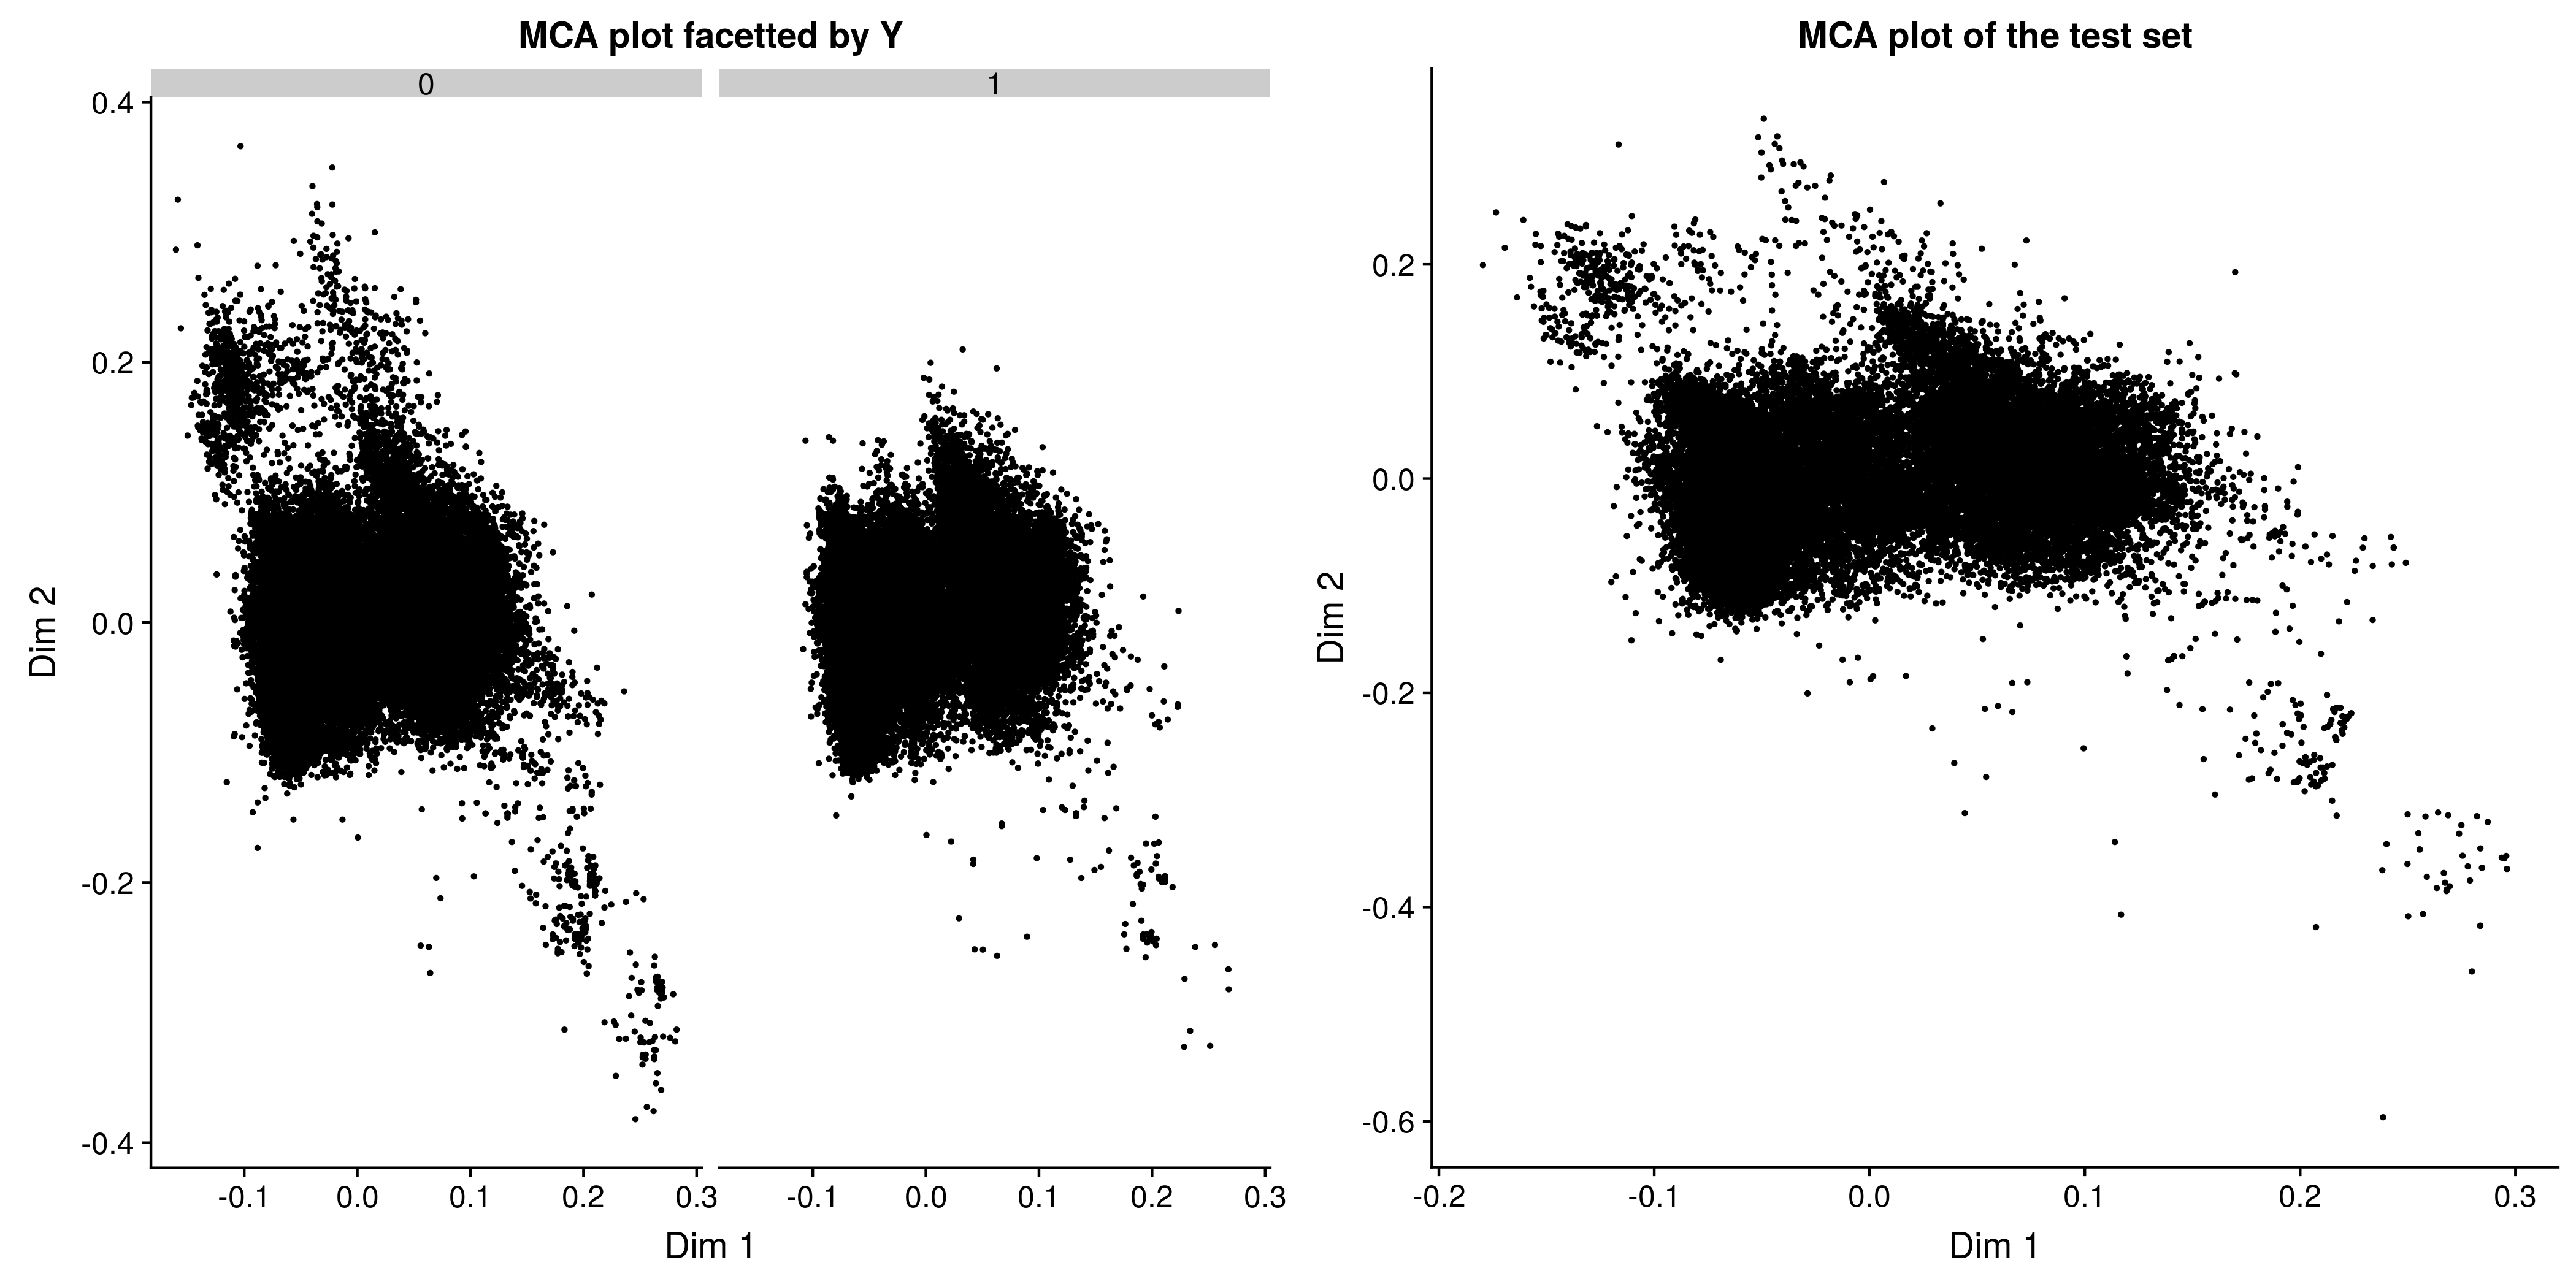
\includegraphics[width=\textwidth]{plots/etiqueta_mca_obs_Y_facet_all}
\end{figure}


\newpage

\setcounter{tocdepth}{2}
\tableofcontents

\newpage
\section{Introduction}

The dataset provided presents a classification problem, whereby the power of several features is to be harnessed to predict a binary label (1/0). A summary of the features available is presented in table \ref{tab:summary}.

\begin{table}[!h]
\centering

\begin{tabular}{r|r|r|r|r|r|r|r|r|r|r}
\hline
binary & counter & edad & etiqueta & farmaco & identificador & nominal & ordinal & raza & sexo & Y\\
\hline
3 & 8 & 1 & 3 & 23 & 1 & 4 & 2 & 1 & 1 & 1\\
\hline
\end{tabular}

\caption{46 features are provided together with an identifier variable (\textit{identificador}) and the label to be predicted \textit{Y}.}
\label{tab:summary}
\end{table}

Y, the target variable, is to be predicted using the information stored in the remaining features by means of (I) a linear model, and (II) a gradient boosting model. But first, the data needs to be preprocessed into a format that suits these algorithms. This is carried out in the R script \texttt{EDA.R}. A guide-through of the code is provided below.

\section{EDA}

\subsection{Load libraries}
\begin{knitrout}
\definecolor{shadecolor}{rgb}{0.969, 0.969, 0.969}\color{fgcolor}\begin{kframe}
\begin{alltt}
\hlkwd{library}\hlstd{(ggplot2)}
\hlkwd{library}\hlstd{(viridis)}
\hlkwd{library}\hlstd{(dplyr)}
\hlkwd{library}\hlstd{(magrittr)}
\hlkwd{library}\hlstd{(waffle)}
\hlkwd{library}\hlstd{(tidyr)}
\hlkwd{library}\hlstd{(tibble)}
\hlkwd{library}\hlstd{(ade4)}
\hlkwd{library}\hlstd{(data.table)}
\hlkwd{library}\hlstd{(stringr)}
\hlkwd{library}\hlstd{(FactoMineR)}
\hlkwd{library}\hlstd{(cowplot)}
\hlkwd{library}\hlstd{(pheatmap)}
\hlkwd{library}\hlstd{(kableExtra)}
\hlcom{# library(MASS) library(scales)}
\hlstd{plot_dir} \hlkwb{<-} \hlstr{"plots"}
\hlstd{output_data} \hlkwb{<-} \hlstr{"proc_data"}
\hlstd{rdata_dir} \hlkwb{<-} \hlstr{"RData"}
\hlstd{tables_dir} \hlkwb{<-} \hlstr{"tables"}
\end{alltt}
\end{kframe}
\end{knitrout}

\subsection{Load data}
Read the \texttt{datos.csv} file and split the training/validation set and the test set.
\begin{knitrout}
\definecolor{shadecolor}{rgb}{0.969, 0.969, 0.969}\color{fgcolor}\begin{kframe}
\begin{alltt}
\hlstd{datos} \hlkwb{<-} \hlkwd{read.table}\hlstd{(}\hlstr{"datos.csv"}\hlstd{,} \hlkwc{sep} \hlstd{=} \hlstr{","}\hlstd{,} \hlkwc{header} \hlstd{= T,} \hlkwc{stringsAsFactors} \hlstd{= F)}
\hlstd{datos} \hlkwb{<-} \hlstd{datos[,} \hlkwd{c}\hlstd{(}\hlkwd{colnames}\hlstd{(datos)[}\hlnum{1}\hlopt{:}\hlnum{4}\hlstd{],} \hlkwd{colnames}\hlstd{(datos)[}\hlnum{5}\hlopt{:}\hlstd{(}\hlkwd{ncol}\hlstd{(datos)} \hlopt{-} \hlnum{1}\hlstd{)]} \hlopt
    \hlstd{sort,} \hlstr{"Y"}\hlstd{)]}
\hlkwd{write}\hlstd{(}\hlkwc{x} \hlstd{=} \hlkwd{kable}\hlstd{(}\hlkwc{x} \hlstd{= datos} \hlopt \hlstd{colnames} \hlopt \hlkwd{strsplit}\hlstd{(.,} \hlkwc{split} \hlstd{=} \hlstr{"_"}\hlstd{)} \hlopt \hlkwd{lapply}\hlstd{(.,}
    \hlkwa{function}\hlstd{(}\hlkwc{x}\hlstd{) x[[}\hlnum{1}\hlstd{]])} \hlopt \hlstd{unlist} \hlopt \hlstd{table} \hlopt \hlstd{t,} \hlkwc{format} \hlstd{=} \hlstr{"latex"}\hlstd{,} \hlkwc{digits} \hlstd{=} \hlnum{2}\hlstd{),}
    \hlkwc{file} \hlstd{=} \hlkwd{file.path}\hlstd{(tables_dir,} \hlstr{"data_summary.tex"}\hlstd{))}


\hlstd{datos}\hlopt{$}\hlstd{edad_integer} \hlkwb{<-} \hlkwd{str_match}\hlstd{(}\hlkwc{string} \hlstd{= datos}\hlopt{$}\hlstd{edad,} \hlkwc{pattern} \hlstd{=} \hlstr{"\textbackslash{}\textbackslash{}[\textbackslash{}\textbackslash{}d\{2\}-(\textbackslash{}\textbackslash{}d\{2\})\textbackslash{}\textbackslash{})"}\hlstd{)} \hlopt
    \hlstd{.[,} \hlnum{2}\hlstd{]} \hlopt \hlstd{as.integer}

\hlstd{train_set} \hlkwb{<-} \hlstd{datos[}\hlopt{!}\hlkwd{is.na}\hlstd{(datos[}\hlstr{"Y"}\hlstd{]), ]}
\hlstd{x_train} \hlkwb{<-} \hlstd{train_set} \hlopt \hlkwd{select}\hlstd{(}\hlopt{-}\hlstd{Y)}
\hlstd{y_train} \hlkwb{<-} \hlkwd{select}\hlstd{(train_set, Y)} \hlopt \hlkwd{mutate}\hlstd{(}\hlkwc{Y} \hlstd{=} \hlkwd{as.factor}\hlstd{(Y))}

\hlstd{test_set} \hlkwb{<-} \hlstd{datos[}\hlkwd{is.na}\hlstd{(datos[}\hlstr{"Y"}\hlstd{]), ]}
\hlstd{x_test} \hlkwb{<-} \hlstd{test_set} \hlopt \hlkwd{select}\hlstd{(}\hlopt{-}\hlstd{Y)}
\end{alltt}
\end{kframe}
\end{knitrout}


\subsection{Visualization of race and age}
A general picture of how the potentially relevant categories race and age dataset are distributed across the individuals is shown in figure \ref{fig:categories}.

  
\begin{figure}[!h]
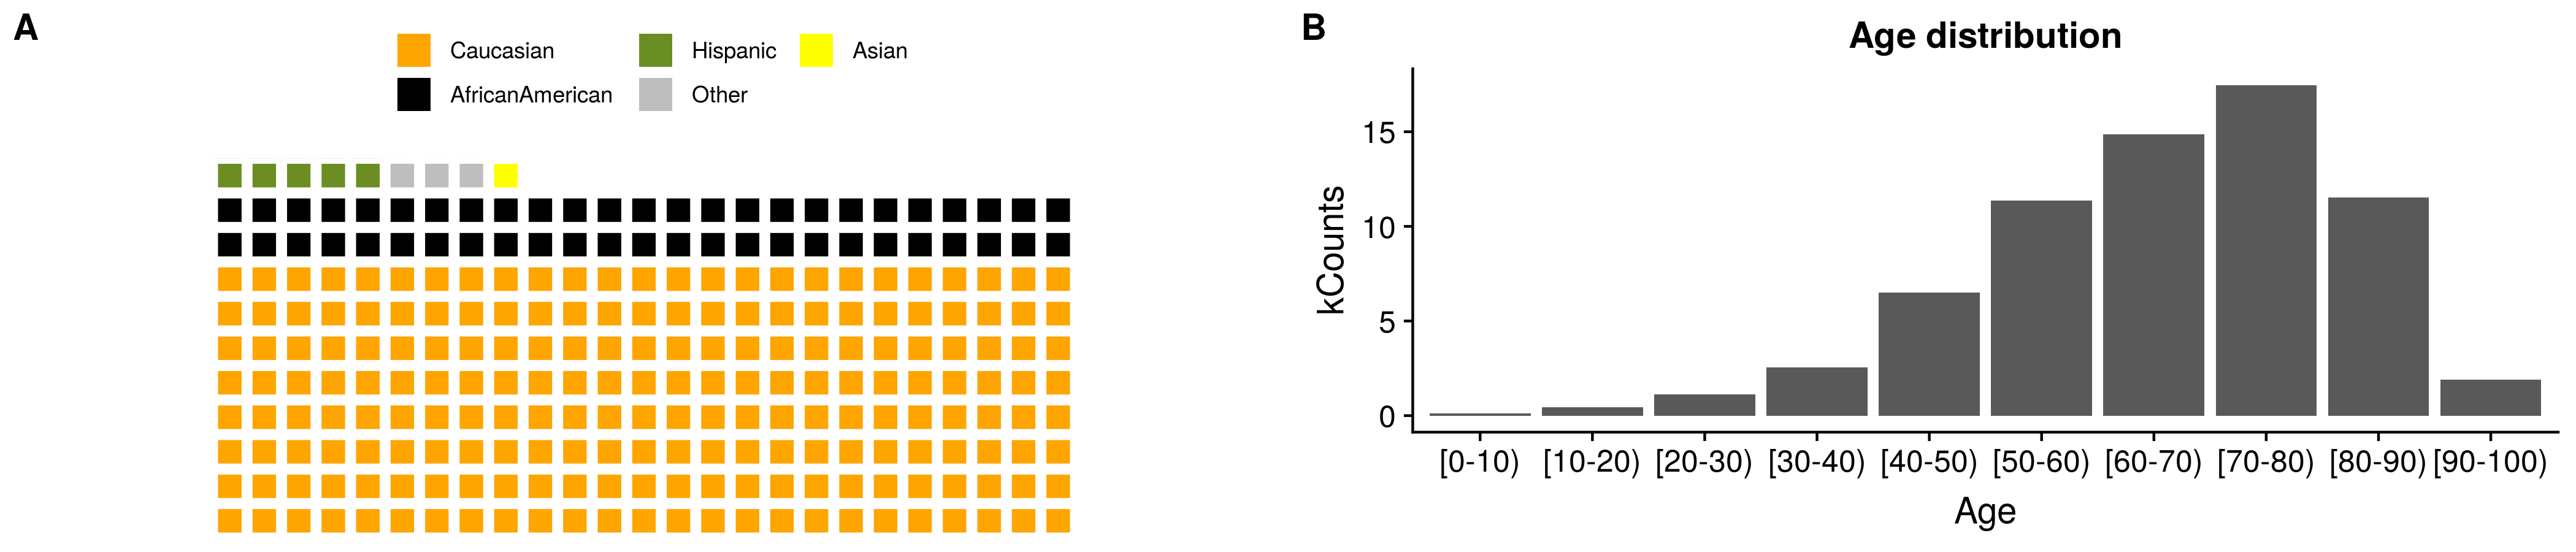
\includegraphics[width=\textwidth]{plots/visualize_categories.png}
\caption{\textbf{A} Waffle plot showing the race distribution. A majority of the individuals are defined as Caucasian, with Afro Americans making up a significant though minor proportion. The remanining individuals are Hispanic, Asian and from other groups. \textbf{B} A histogram over the age groups reveals a trend for individuals to be aged 50 and 90 years old.}
\label{fig:categories}
\end{figure}
  
The non uniform distribution of individuals over these categories and eventually many others showcases the existence of some bias in the data.

\subsection{Preprocess the training and test sets}

Define a function to preprocess the train dataset and prepare it for the machine learning algorithms. The test set will follow a preprocessing parallel to the train

\begin{itemize}
\item Numerical variabels stay the same (quantitative)
\item Ordinal variables (categories with order) stay the same (quantitative)
\item Farmacos are considered ordinals (quantitative)
\item Nominal variables (categories with no defined order) are reformatted to one-hot (qualitiative)
\item Binary stays the same (qualitiative)
\item Race is reformatted to one-hot (qualitiative)
\item Sex stays the same (only made into 1/0) (qualitiative)
\item Etiquetas. There is room for 3 etiquetas, but it is only their presence that matters. Therefore they are passed to one-hot encoding. The i,j cell will store how many times the jth etiqueta is present in the ith sample i.e. 0 to 3 times if it appears in none or 3 slots, respectively (qualitiative)
\end{itemize}

Once the function is defined, it was applied to preprocess the training and test datasets in parallel. See appendix B for source code.

  
\subsection{\textbf{P}rincipal \textbf{C}omponent \textbf{A}nalysis (PCA)}

The distribution of edad (age), raza (race), gender (sexo) and Y (label) across individuals on the 2D plane capturing the most variance can be visualized by means of a PCA. The PCA takes numerical features and rotates them into a new space where variance (information) is maximised on each new feature (principal component). The first two can be used to generate the mentioned 2D plane. This is shown in figure \ref{fig:pca_multicategory}

\begin{figure}[!h]
\centering
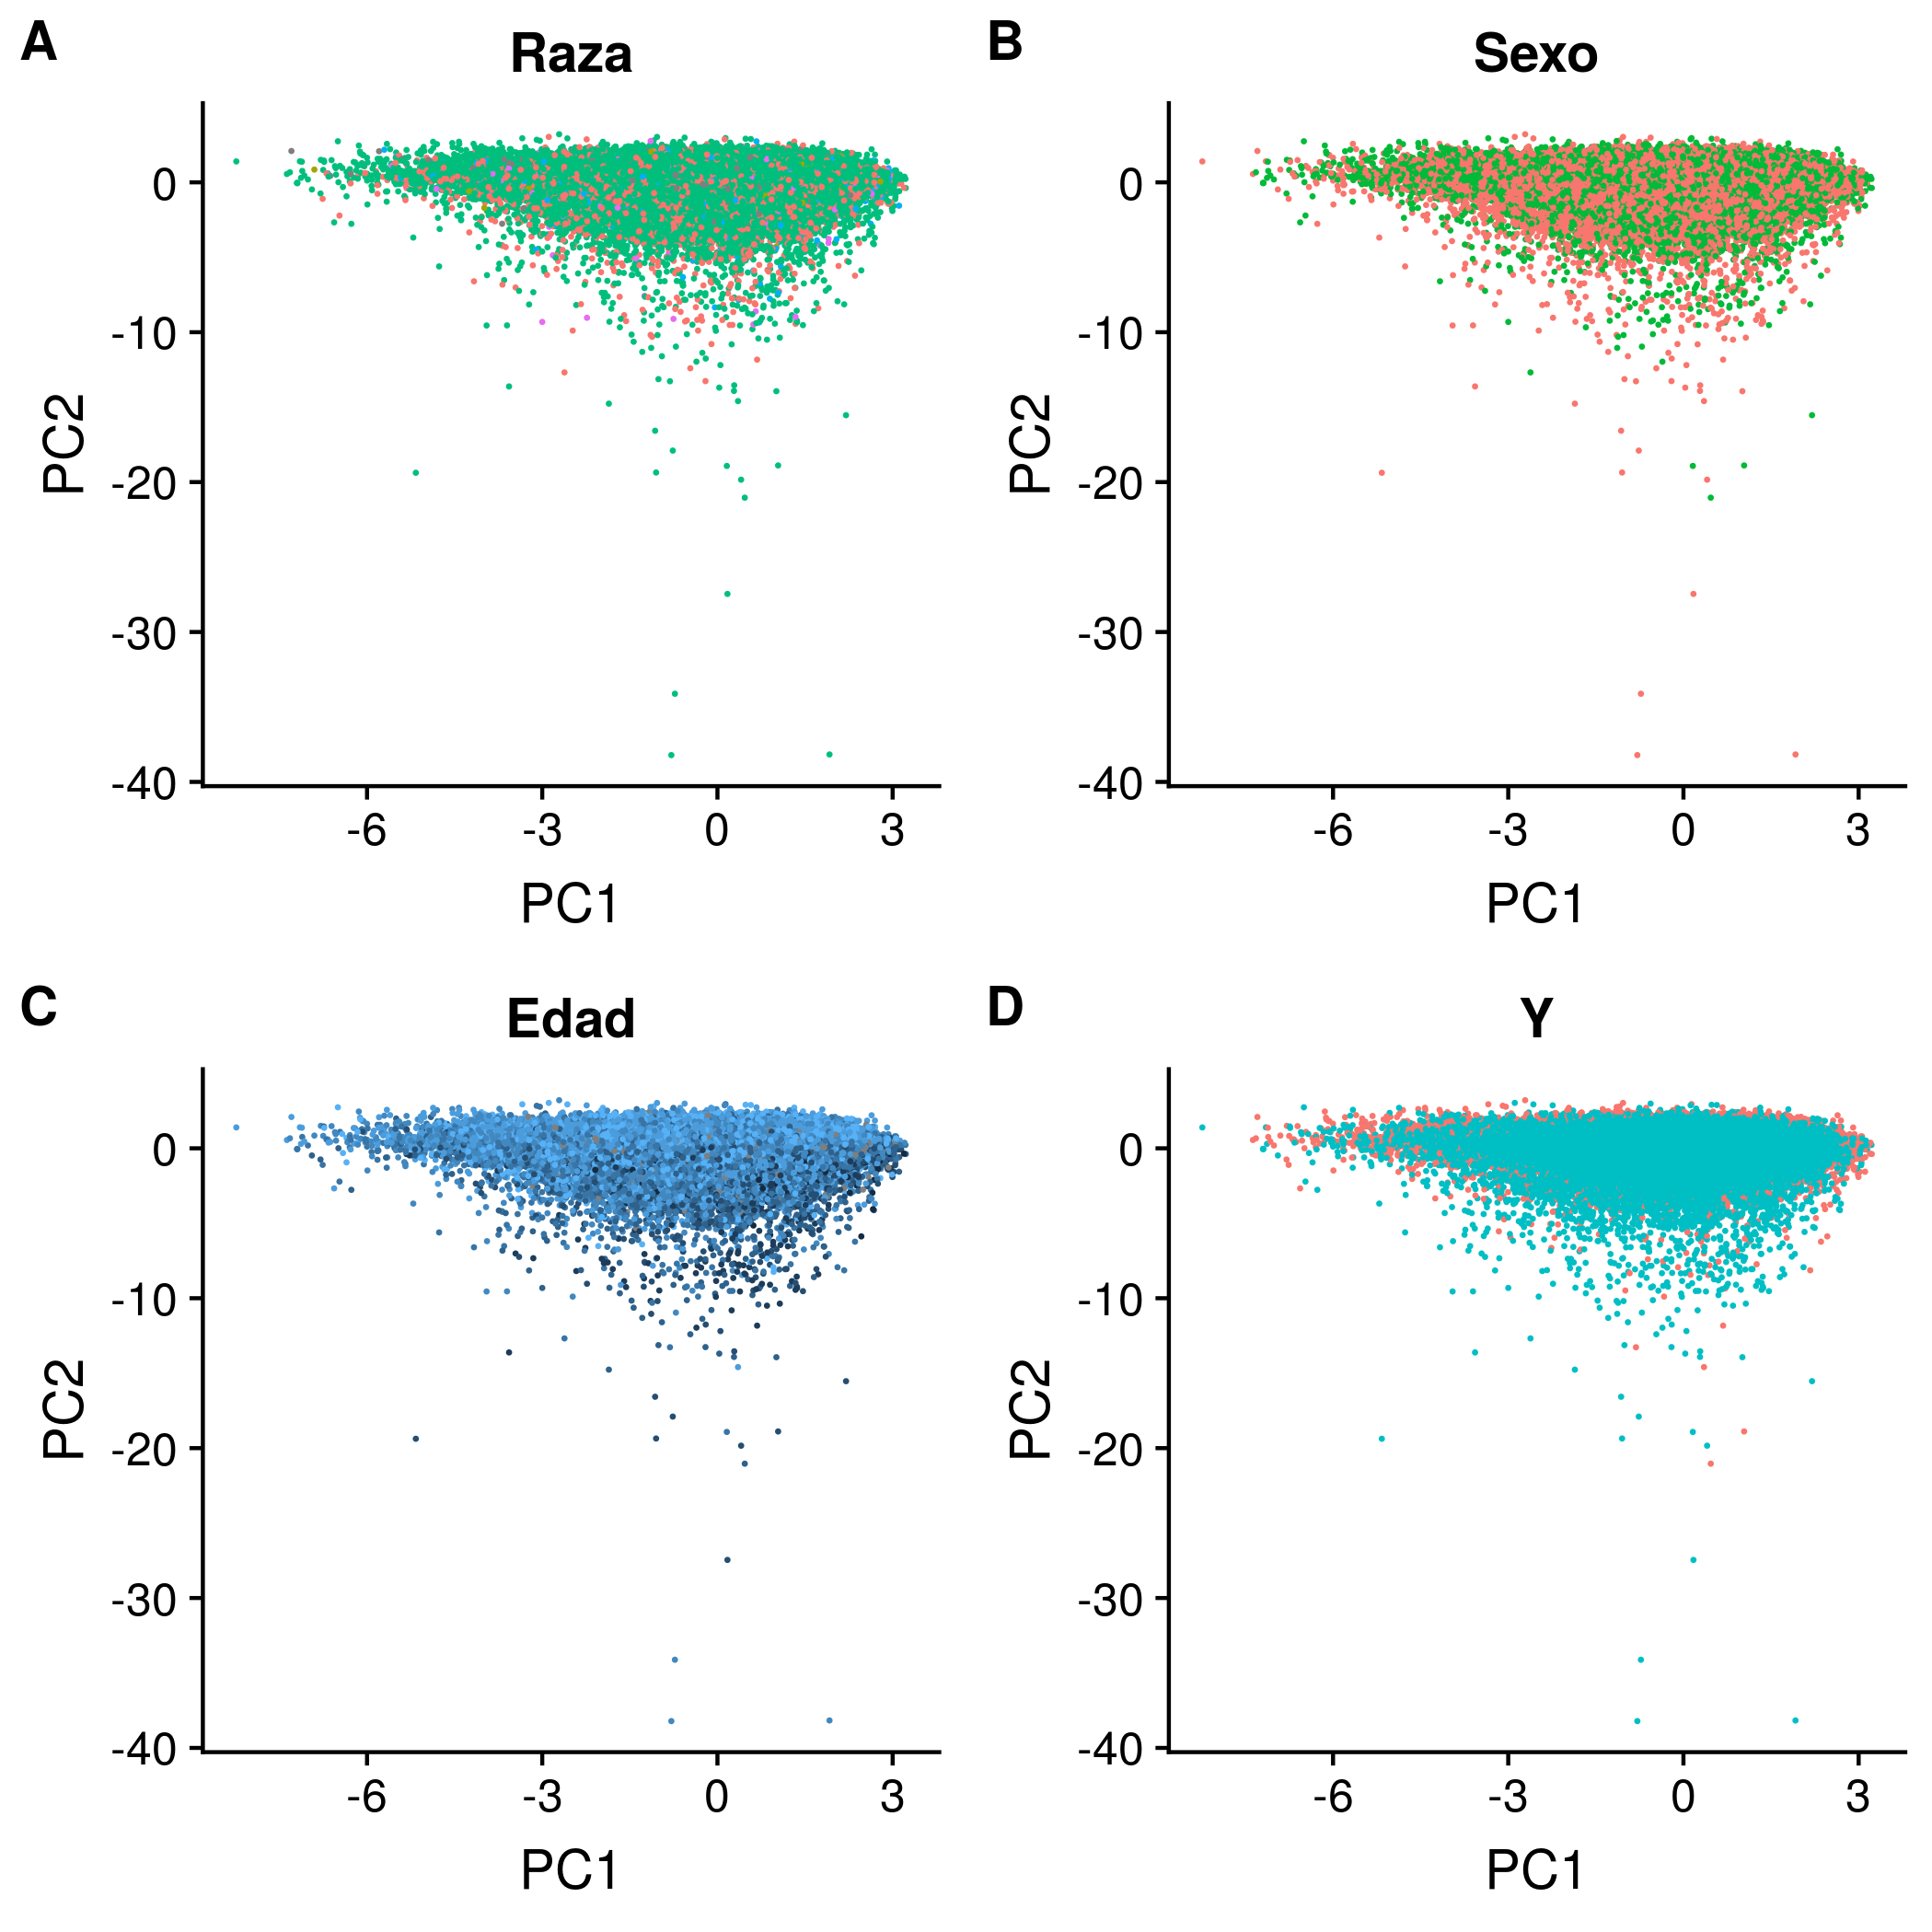
\includegraphics[width=\textwidth]{plots/PCA_multicategory}
\caption{PCA plots for individuals colored by race, gender, age and label. No category seems to be distinguishable on the 2D plane in any of the features probed.}
\label{fig:pca_multicategory}
\end{figure}

The PCA did not successfully evidence any clear pattern.

\subsection{\textbf{M}ultiple \textbf{C}orrespondence \textbf{A}nalysis (MCA)}

An analogous analysis can be performed using categorical variables with the MCA algorithm from the R package FactoMineR. The algorithm was run with and without etiquetas (tags) to explore if saving these ensemble of one-hot features could be spared for computational efficiency. A plot of the contribution of the explored variables to the new 2D plane is shown in figure \ref{fig:mca_variables}, whereas a plot of the individuals in this plane is shown on figure \ref{fig:mca_obs_Y}.

\begin{figure}[!h]
\centering
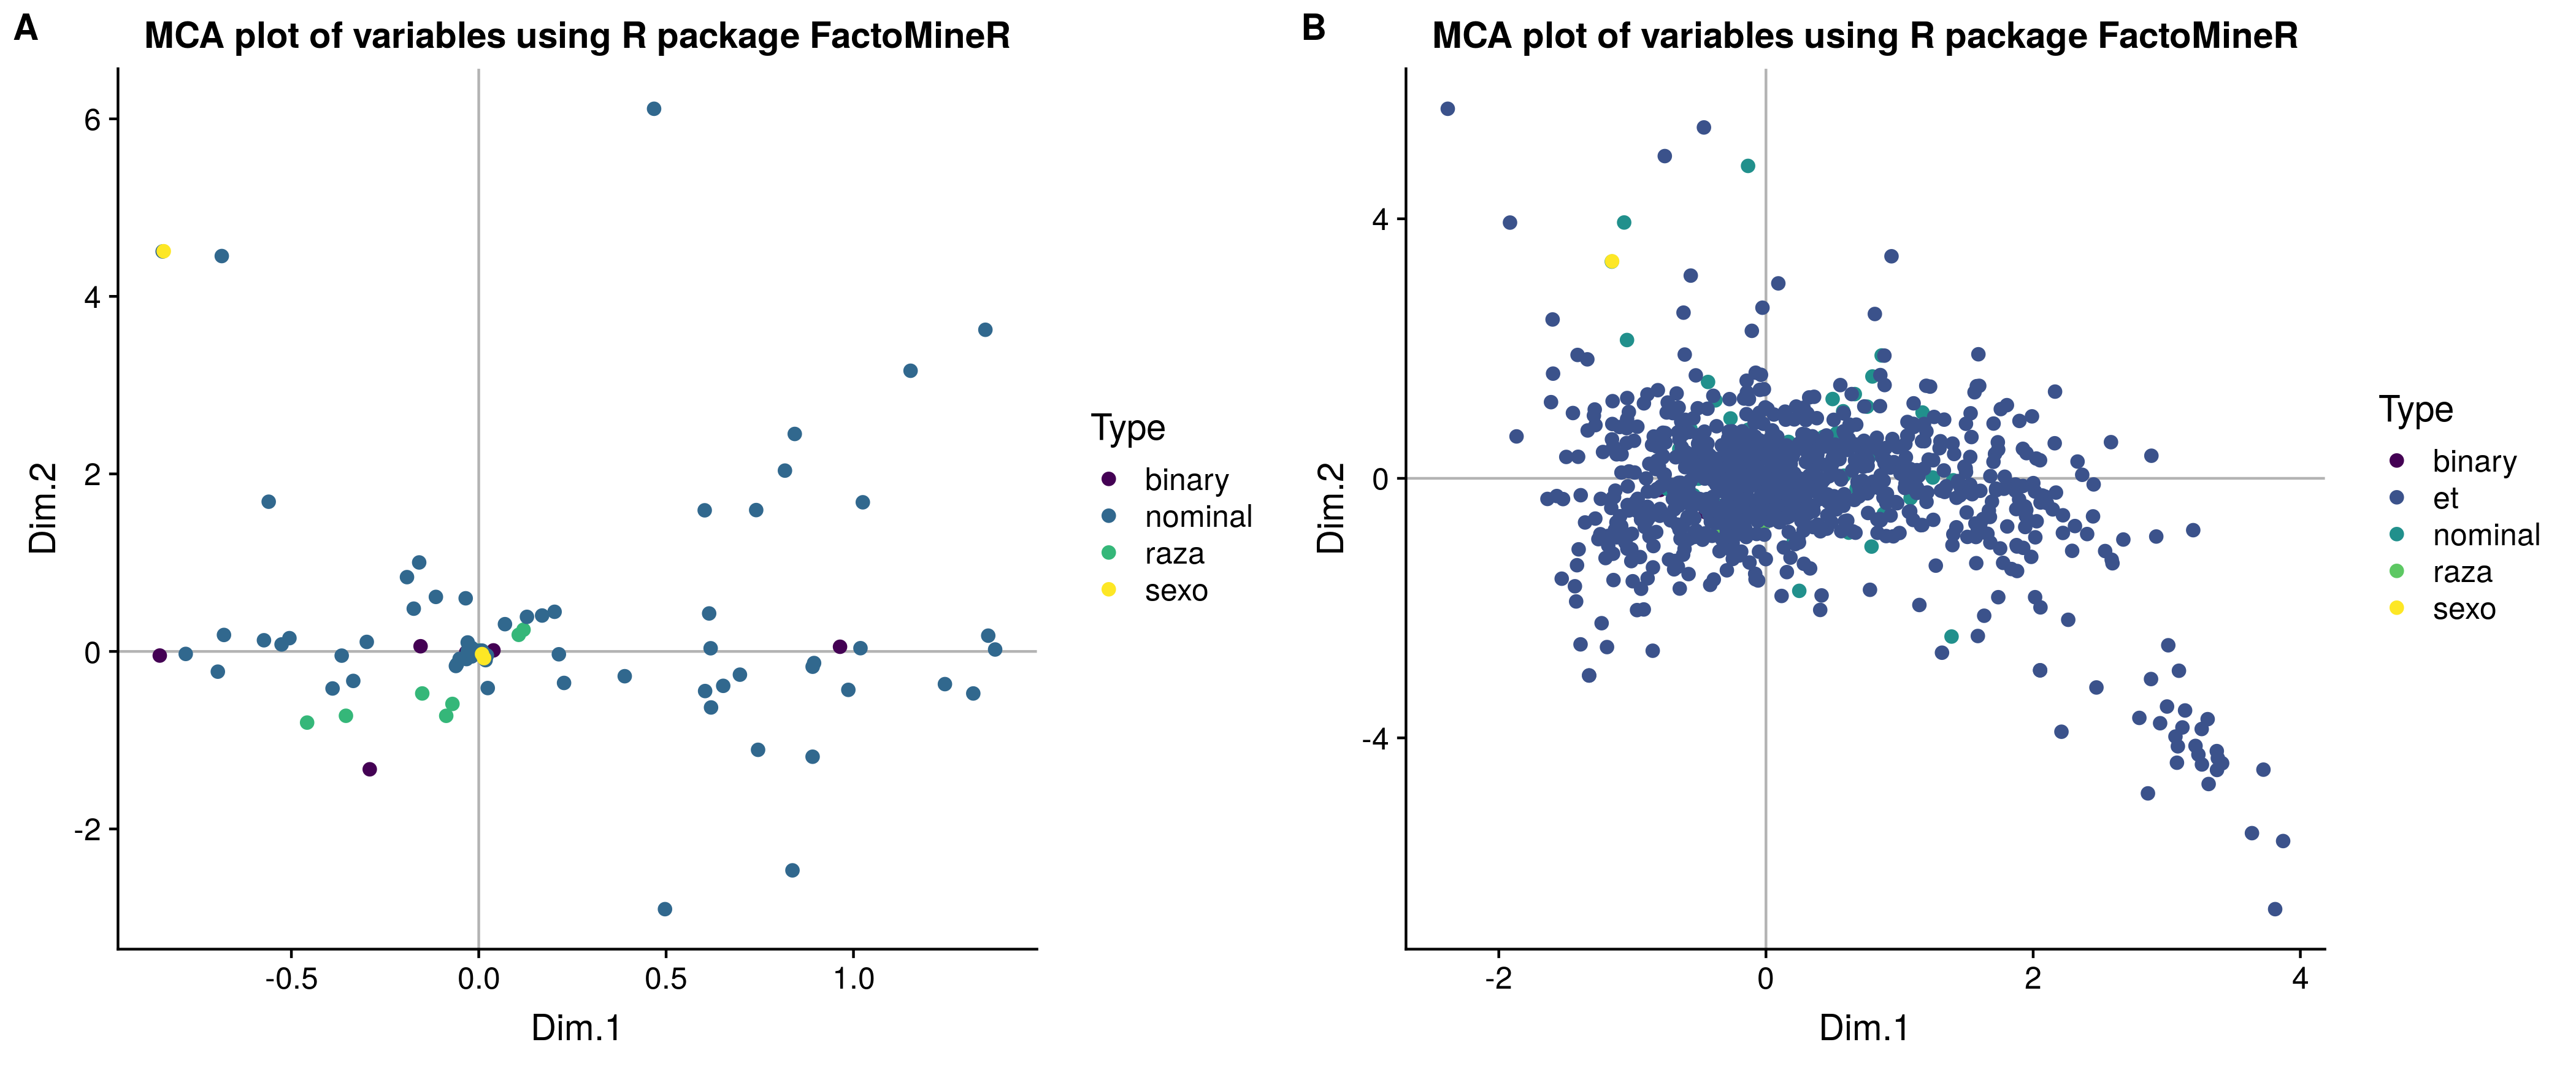
\includegraphics[width=0.7\textwidth]{plots/mca_variables_combined}
\caption{Visualization of the contribution of each categorical variable to the most informative MCA 2D plane. Etiquetas and nominal variables seemed to bring the most information. \textbf{A} Without etiquetas. \textbf{B} With etiquetas.}
\label{fig:mca_variables}
\end{figure}

\begin{figure}[!h]
\centering
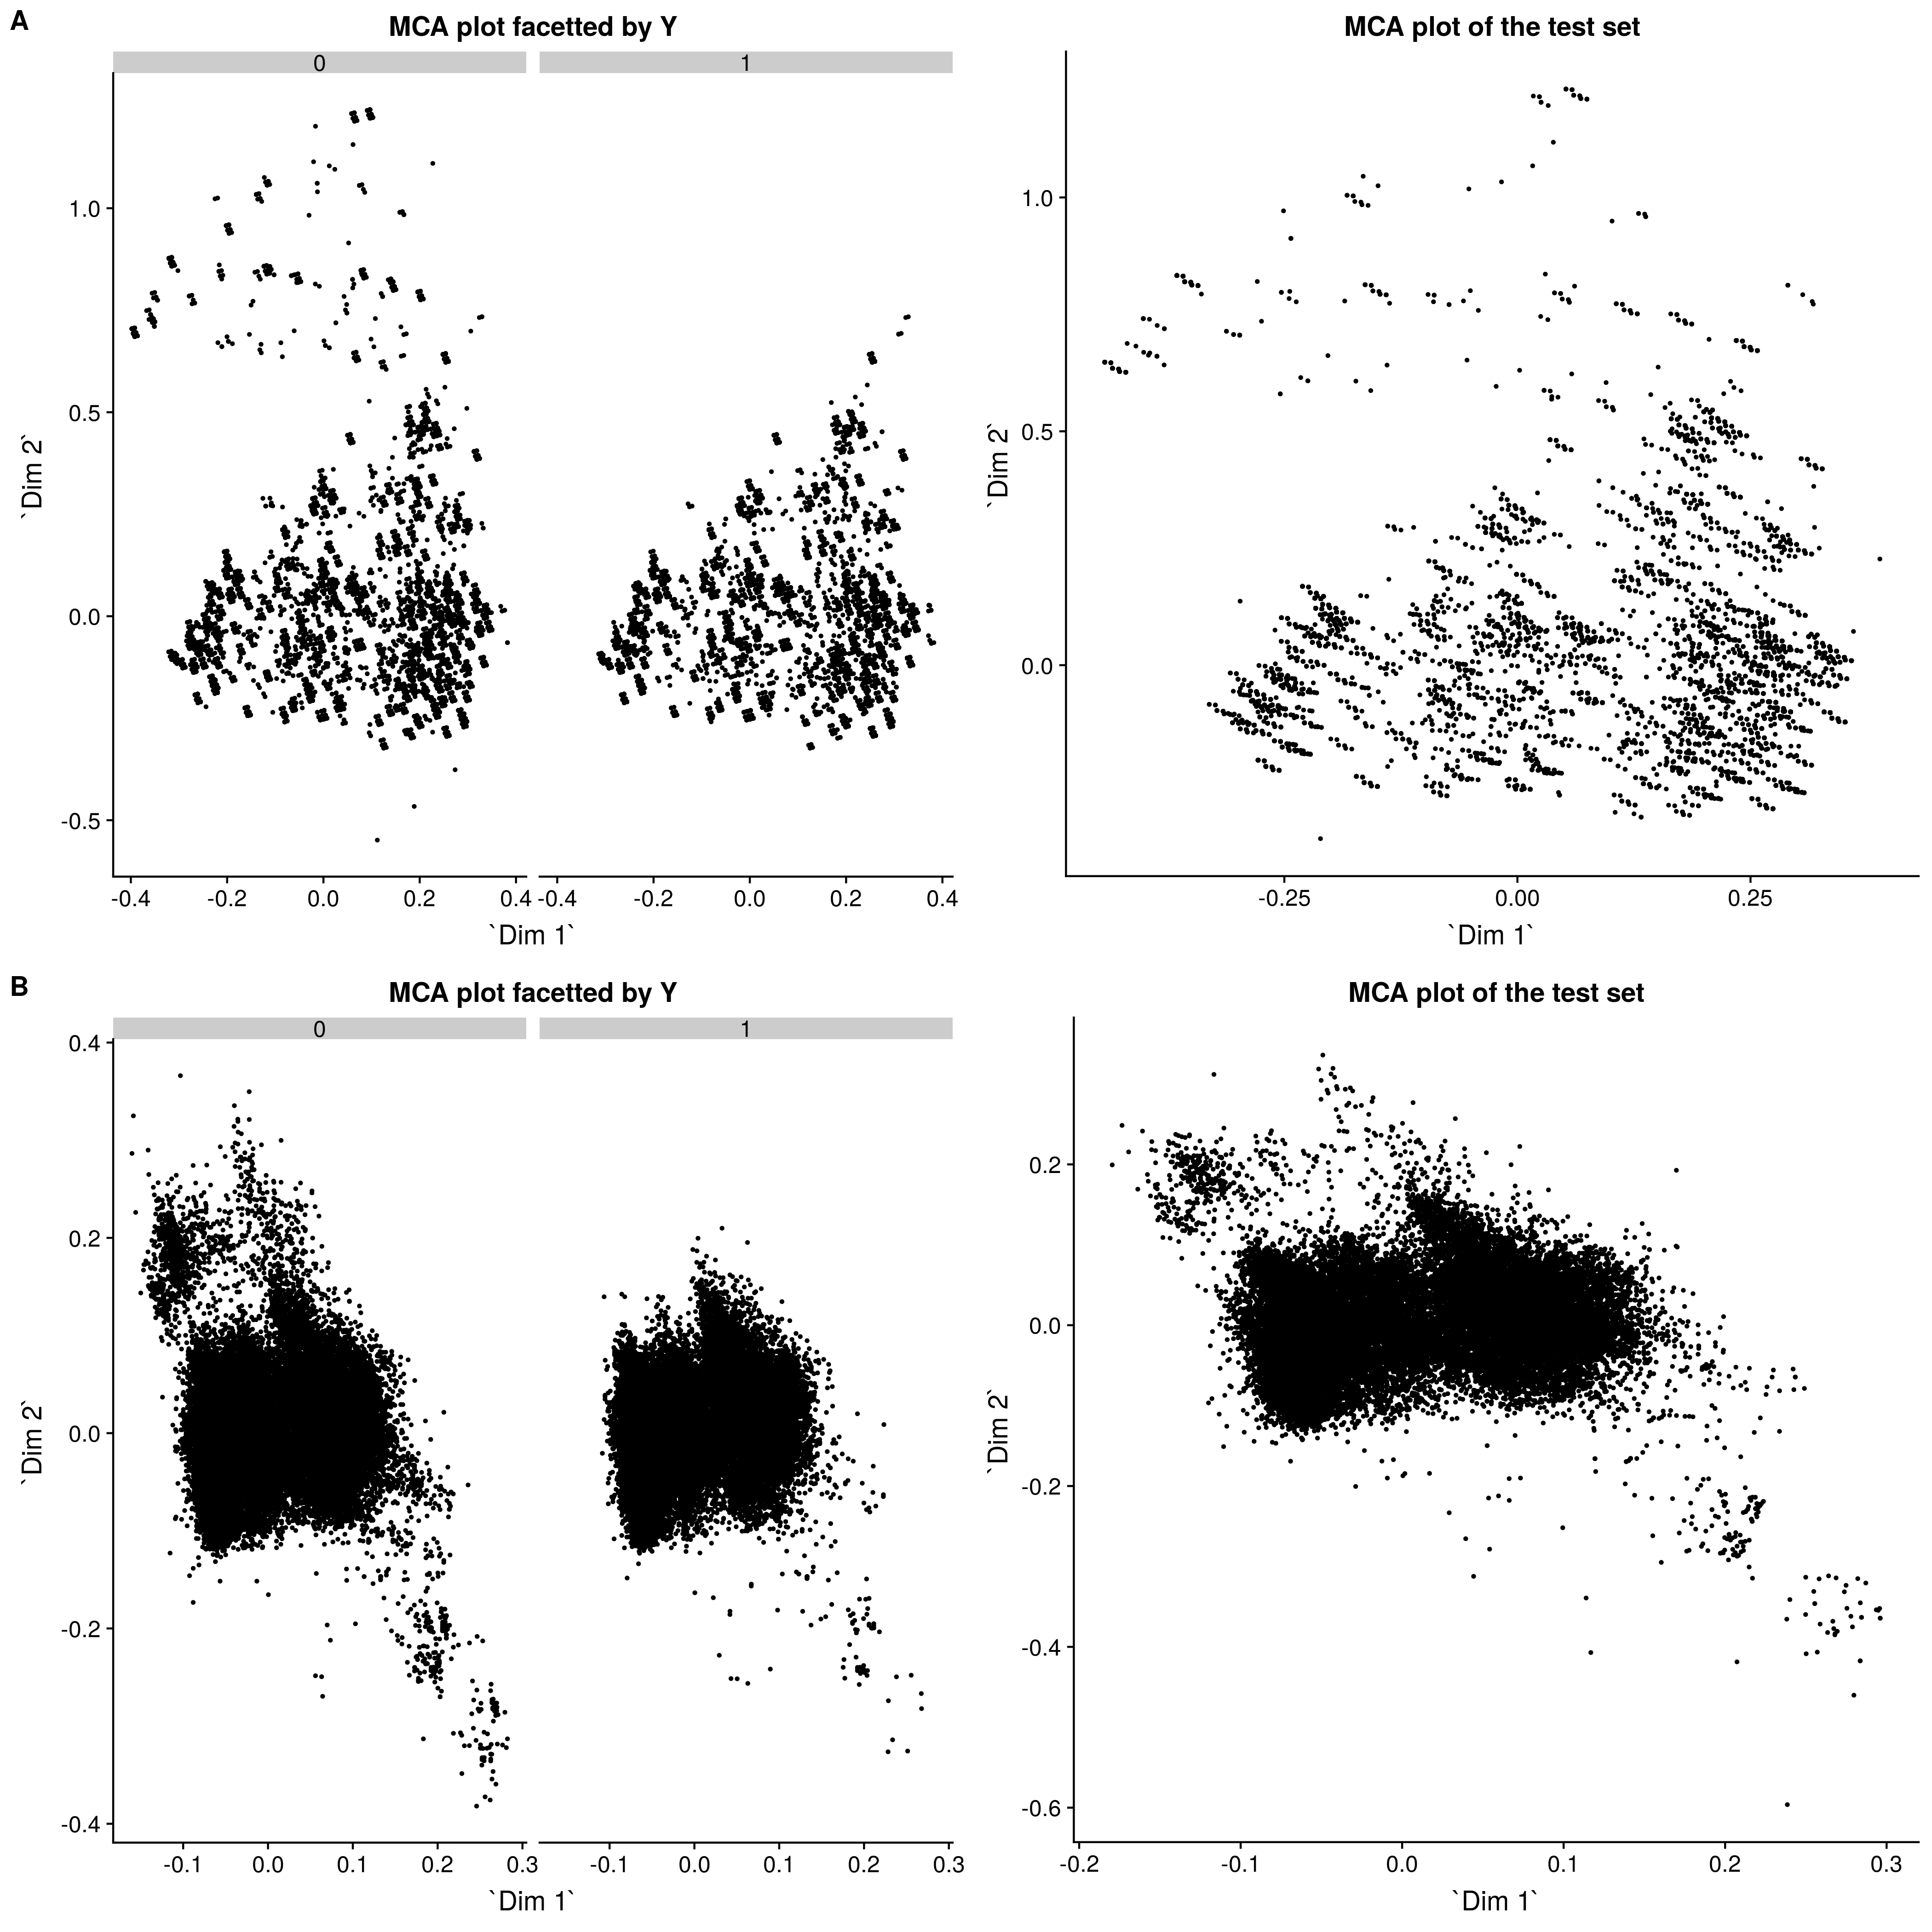
\includegraphics[width=0.7\textwidth]{plots/mca_obs_Y_facet_all_combined}
\caption{A visualization of the individuals on the MCA 2D plane facetted by label. A clear separation is visible for some individuals, clustering around the top left corner of the plot. A very similar pattern is observed in the test set. \textbf{A} Without etiquetas. \textbf{B} With etiquetas.}
\label{fig:mca_obs_Y}
\end{figure}

The analysis, whose results are shown in figures the mentioned figures, is able to successfuly find a pattern whereby individuals clustering in the top left corner are highly likely to be of class 0 (Y=0). The features extracted in this analysis will be added to the processed data in order to make use of their predictive power in the model training. Remarkably, if MCA is conducted without etiquetas, many individuals are projected on the same spot of the 2D plane. This effect is canceled when etiquetas are included, indicating that indeed etiquetas contribute to each of the individuals' diversity. For this reason, the top 5 MCA features produced when including etiquetas will be used to power the models. Figure \ref{fig:mca_contrib} shows the single greatest contributions come from nominal variables, even though the whole of the etiquetas might contribute more in the end, given the sheer amount of etiquetas.


\begin{figure}[!h]
\centering
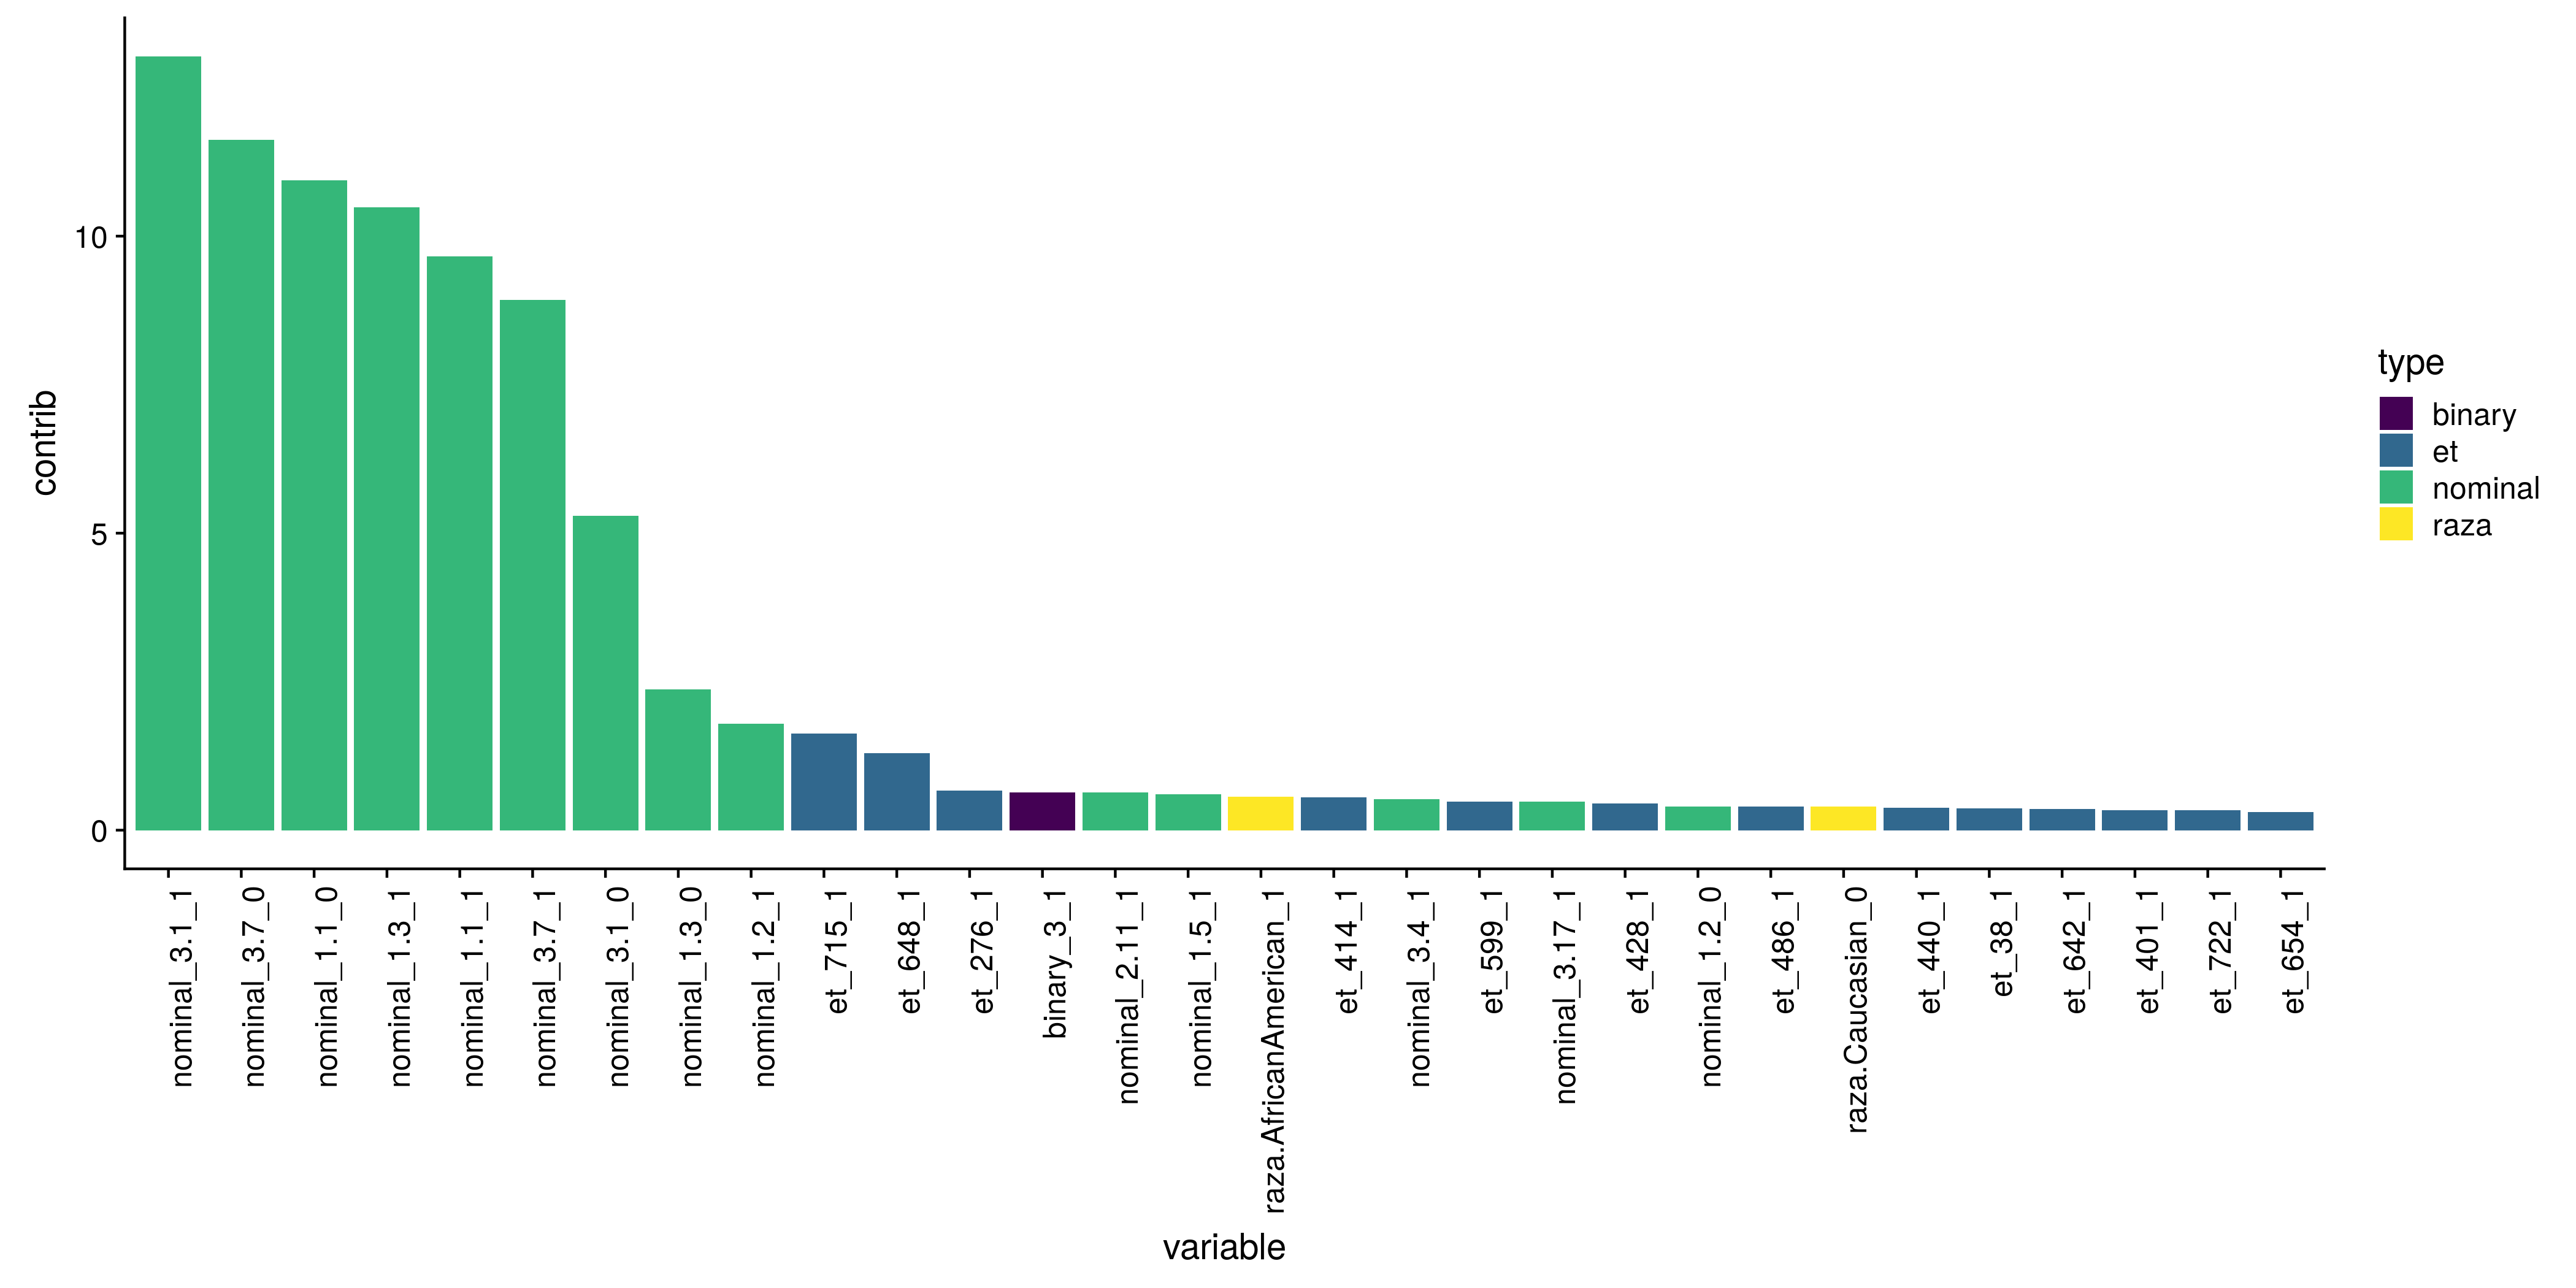
\includegraphics[width=0.7\textwidth]{plots/etiqueta_mca_contrib}
\caption{Top 30 variables contributing to the overall variance found by the MCA ordered by its size and coloured by type.}
\label{fig:mca_contrib}
\end{figure}
\subsection{Heatmap}

Finally, a heatmap (figure \ref{fig:heatmap}) is an alternative way to visualize the presence of any patterns/clustering in the processed dataset.

\begin{figure}[!h]
\centering
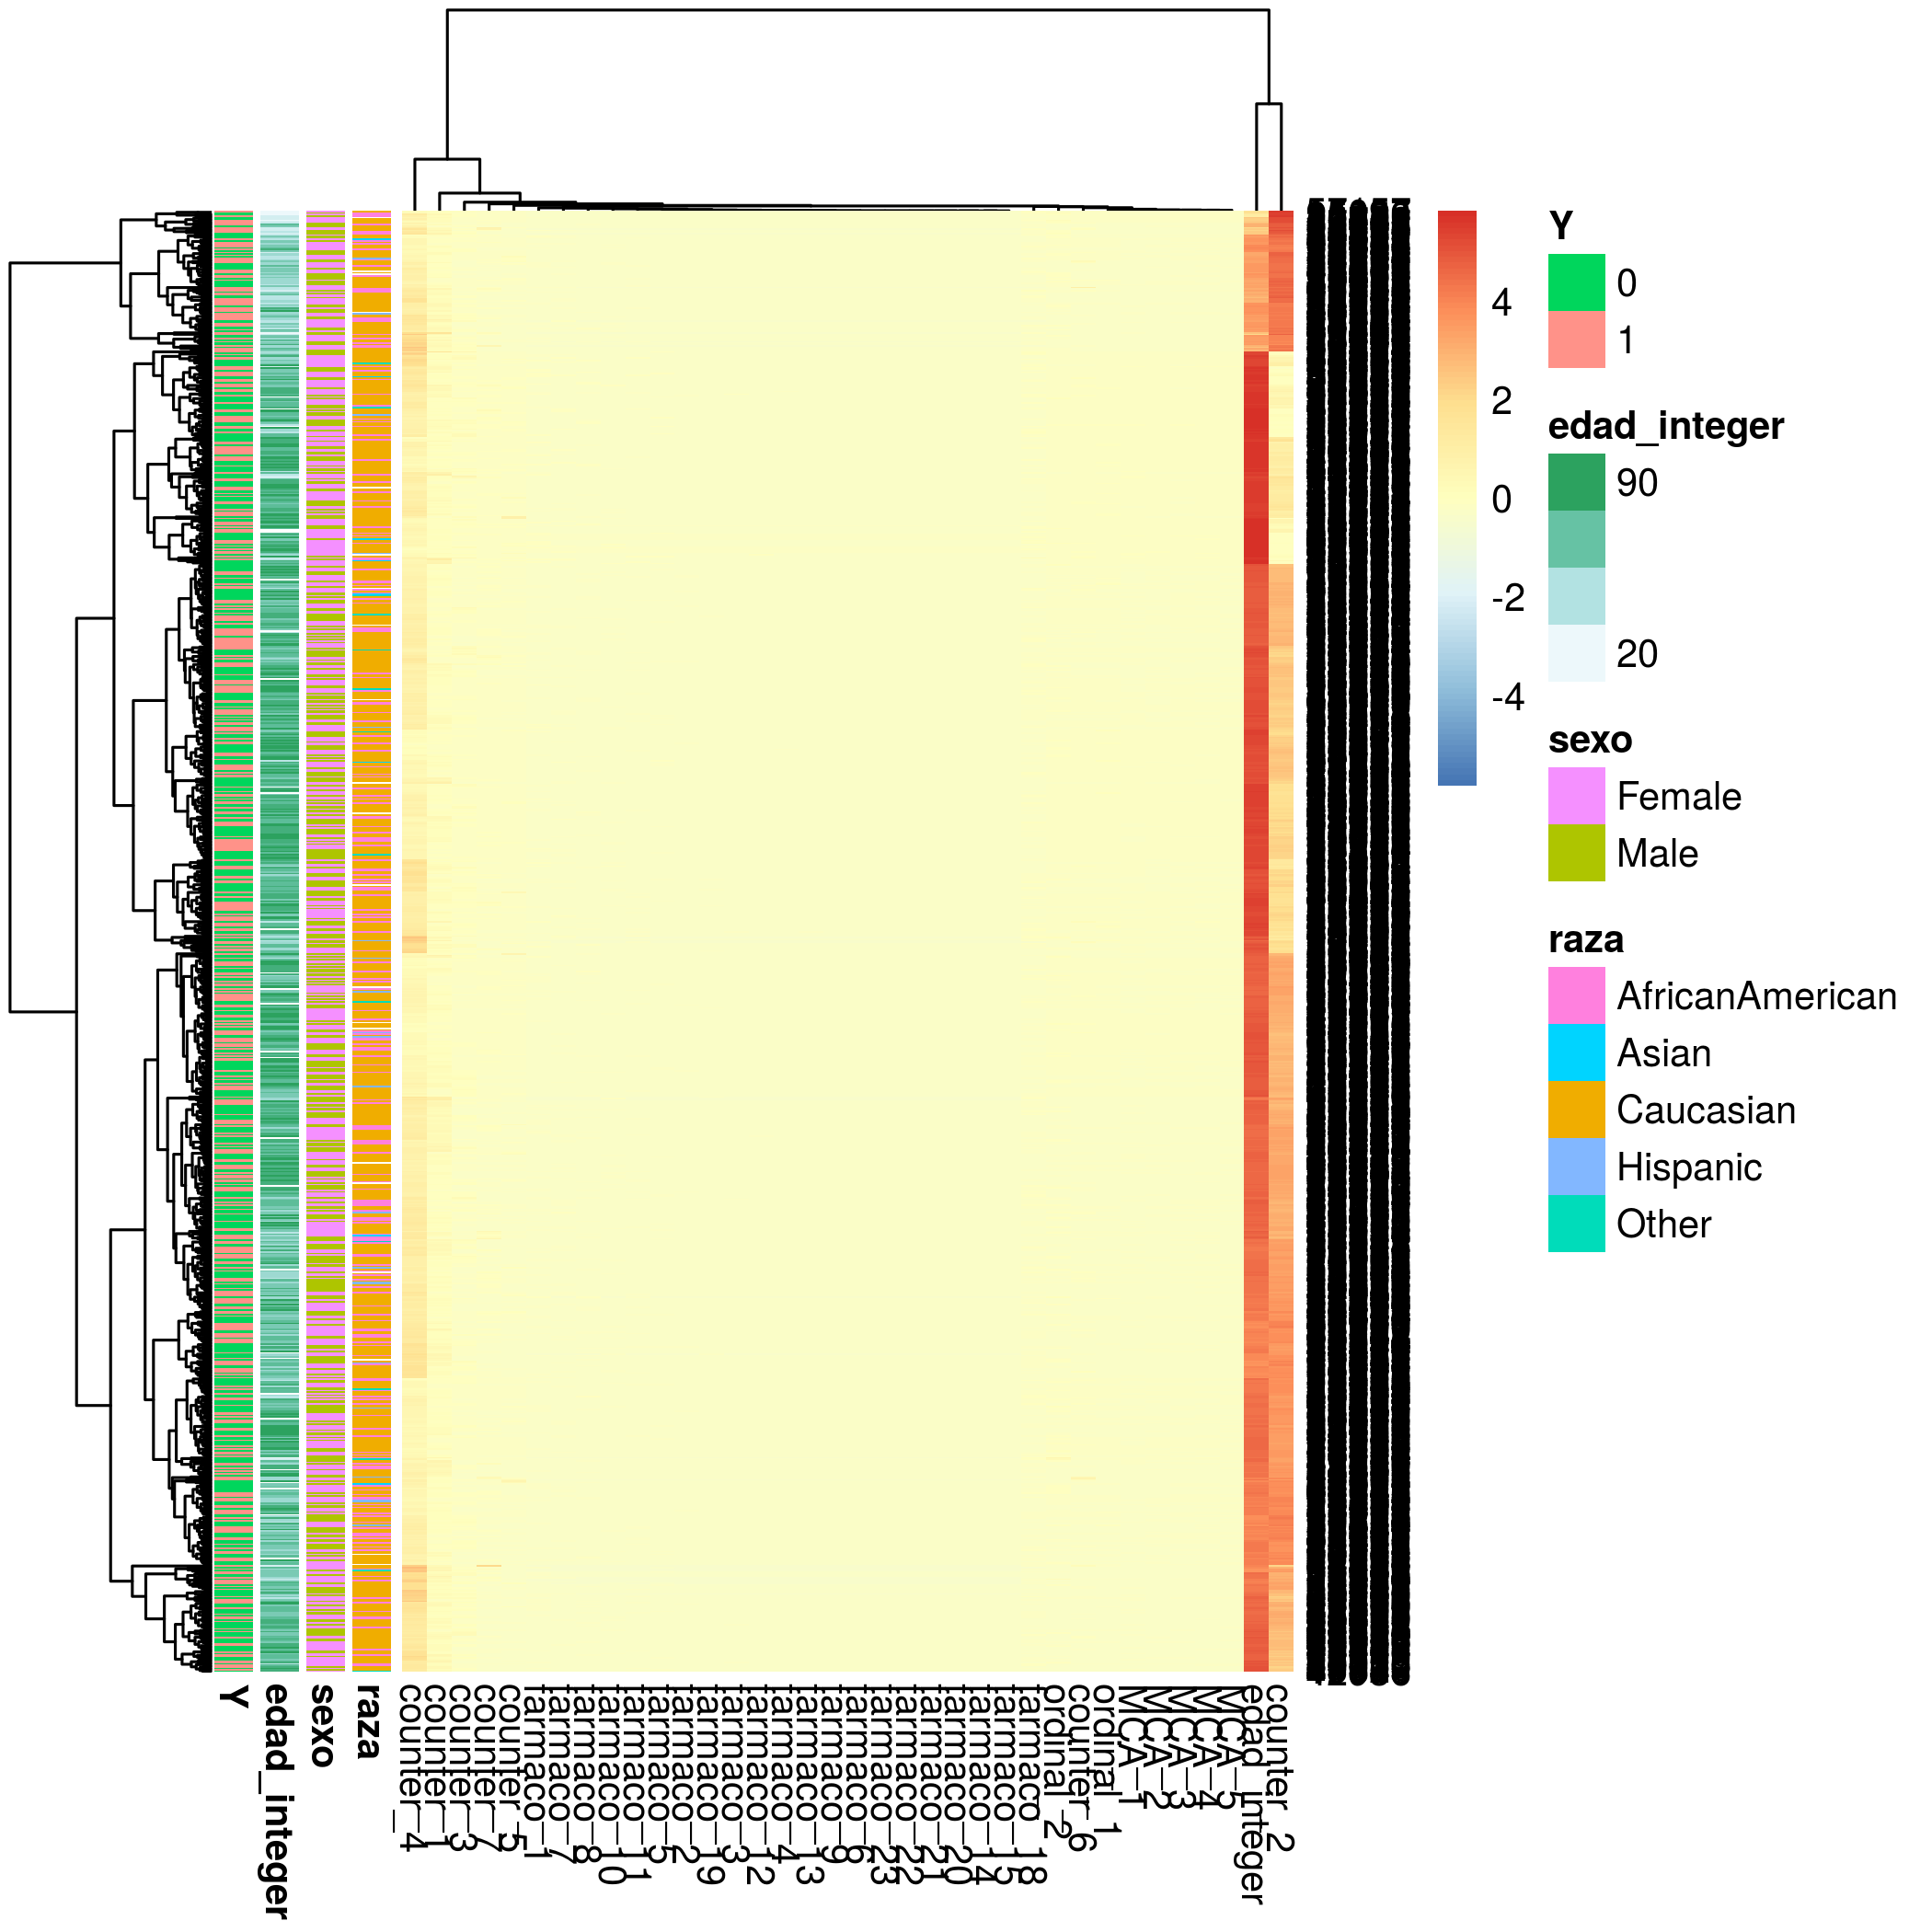
\includegraphics[width=0.7\textwidth]{plots/heatmap}
\caption{Heatmap of the training set including the top 5 MCA features. As expected, age and the counters with the most levels/categories are the first splitting features. However, the MCA features don't seem to contribute to the clustering.}
\label{fig:heatmap}
\end{figure}

\subsection{Improvements to the EDA}

More insights could be extracted by performing supervised projections of the dataset, where new highly informative planes are found taking into account the label. Moreover, more intensive processing, like the usage of an autoencoder, could be used to perform more powerful dimensionality reduction on the categorical variables, specially the etiquetas.

\subsection{Export features}
\begin{knitrout}
\definecolor{shadecolor}{rgb}{0.969, 0.969, 0.969}\color{fgcolor}\begin{kframe}
\begin{alltt}
\hlcom{# Save processed datasets without one-hot encoding data but with mca features}
\hlkwd{write.table}\hlstd{(}\hlkwc{x} \hlstd{= train_sup_proj_data}\hlopt{$}\hlstd{proj,} \hlkwc{file} \hlstd{=} \hlkwd{file.path}\hlstd{(output_data,} \hlstr{"x_train_mca.csv"}\hlstd{),}
    \hlkwc{sep} \hlstd{=} \hlstr{","}\hlstd{,} \hlkwc{row.names} \hlstd{= x_train}\hlopt{$}\hlstd{identificador,} \hlkwc{quote} \hlstd{= F,} \hlkwc{col.names} \hlstd{= T)}
\hlkwd{write.table}\hlstd{(}\hlkwc{x} \hlstd{= test_sup_proj_data}\hlopt{$}\hlstd{proj,} \hlkwc{file} \hlstd{=} \hlkwd{file.path}\hlstd{(output_data,} \hlstr{"x_test_mca.csv"}\hlstd{),}
    \hlkwc{sep} \hlstd{=} \hlstr{","}\hlstd{,} \hlkwc{row.names} \hlstd{= x_test}\hlopt{$}\hlstd{identificador,} \hlkwc{quote} \hlstd{= F,} \hlkwc{col.names} \hlstd{= T)}

\hlkwd{write.table}\hlstd{(}\hlkwc{x} \hlstd{= train_sup_proj_data_full}\hlopt{$}\hlstd{proj,} \hlkwc{file} \hlstd{=} \hlkwd{file.path}\hlstd{(output_data,} \hlstr{"x_train_mca_full.csv"}\hlstd{),}
    \hlkwc{sep} \hlstd{=} \hlstr{","}\hlstd{,} \hlkwc{row.names} \hlstd{= x_train}\hlopt{$}\hlstd{identificador,} \hlkwc{quote} \hlstd{= F,} \hlkwc{col.names} \hlstd{= T)}
\hlkwd{write.table}\hlstd{(}\hlkwc{x} \hlstd{= test_sup_proj_data_full}\hlopt{$}\hlstd{proj,} \hlkwc{file} \hlstd{=} \hlkwd{file.path}\hlstd{(output_data,} \hlstr{"x_test_mca_full.csv"}\hlstd{),}
    \hlkwc{sep} \hlstd{=} \hlstr{","}\hlstd{,} \hlkwc{row.names} \hlstd{= x_test}\hlopt{$}\hlstd{identificador,} \hlkwc{quote} \hlstd{= F,} \hlkwc{col.names} \hlstd{= T)}

\hlcom{# Save label to a separate file}
\hlkwd{write.table}\hlstd{(}\hlkwc{x} \hlstd{= y_train,} \hlkwc{file} \hlstd{=} \hlkwd{file.path}\hlstd{(output_data,} \hlstr{"y_train.csv"}\hlstd{),} \hlkwc{sep} \hlstd{=} \hlstr{","}\hlstd{,}
    \hlkwc{row.names} \hlstd{= x_train}\hlopt{$}\hlstd{identificador,} \hlkwc{quote} \hlstd{= F,} \hlkwc{col.names} \hlstd{= T)}
\end{alltt}
\end{kframe}
\end{knitrout}

\section{Session info}
\begin{itemize}
\item 12 GB RAM
\item 8 processors Intel(R) Core(TM) i7-6700HQ CPU at 2.60GHz
\end{itemize}

\begin{knitrout}
\definecolor{shadecolor}{rgb}{0.969, 0.969, 0.969}\color{fgcolor}\begin{kframe}
\begin{alltt}
\hlkwd{sessionInfo}\hlstd{()}
\end{alltt}
\begin{verbatim}
## R version 3.4.4 (2018-03-15)
## Platform: x86_64-pc-linux-gnu (64-bit)
## Running under: Ubuntu 16.04.5 LTS
## 
## Matrix products: default
## BLAS: /usr/lib/openblas-base/libblas.so.3
## LAPACK: /usr/lib/libopenblasp-r0.2.18.so
## 
## locale:
##  [1] LC_CTYPE=en_US.UTF-8       LC_NUMERIC=C              
##  [3] LC_TIME=es_ES.UTF-8        LC_COLLATE=en_US.UTF-8    
##  [5] LC_MONETARY=es_ES.UTF-8    LC_MESSAGES=en_US.UTF-8   
##  [7] LC_PAPER=es_ES.UTF-8       LC_NAME=C                 
##  [9] LC_ADDRESS=C               LC_TELEPHONE=C            
## [11] LC_MEASUREMENT=es_ES.UTF-8 LC_IDENTIFICATION=C       
## 
## attached base packages:
## [1] stats     graphics  grDevices utils     datasets  methods   base     
## 
## other attached packages:
##  [1] kableExtra_0.9.0  pheatmap_1.0.10   cowplot_0.9.2     FactoMineR_1.41  
##  [5] stringr_1.3.1     data.table_1.11.8 ade4_1.7-11       tibble_1.4.2     
##  [9] tidyr_0.8.1       waffle_0.8.0      magrittr_1.5      dplyr_0.7.7      
## [13] viridis_0.5.1     viridisLite_0.3.0 ggplot2_3.1.0     knitr_1.20       
## 
## loaded via a namespace (and not attached):
##  [1] tidyselect_0.2.5     purrr_0.2.5          lattice_0.20-35     
##  [4] colorspace_1.3-2     htmltools_0.3.6      rlang_0.3.0.1       
##  [7] pillar_1.3.0         glue_1.3.0           withr_2.1.2         
## [10] RColorBrewer_1.1-2   bindrcpp_0.2.2       bindr_0.1.1         
## [13] plyr_1.8.4           munsell_0.5.0        gtable_0.2.0        
## [16] rvest_0.3.2          codetools_0.2-15     leaps_3.0           
## [19] evaluate_0.10.1      extrafont_0.17       curl_3.2            
## [22] Rttf2pt1_1.3.6       highr_0.7            Rcpp_0.12.19        
## [25] readr_1.1.1          scales_1.0.0.9000    backports_1.1.2     
## [28] flashClust_1.01-2    formatR_1.5          scatterplot3d_0.3-41
## [31] gridExtra_2.3        hms_0.4.2            digest_0.6.18       
## [34] stringi_1.2.4        grid_3.4.4           rprojroot_1.3-2     
## [37] tools_3.4.4          lazyeval_0.2.1       cluster_2.0.7-1     
## [40] crayon_1.3.4         extrafontdb_1.0      pkgconfig_2.0.2     
## [43] MASS_7.3-48          xml2_1.2.0           httr_1.3.1          
## [46] rstudioapi_0.8       assertthat_0.2.0     rmarkdown_1.10      
## [49] R6_2.3.0             compiler_3.4.4
\end{verbatim}
\end{kframe}
\end{knitrout}

\newpage
\section{Appendix A}

\begin{figure}[!h]
\centering
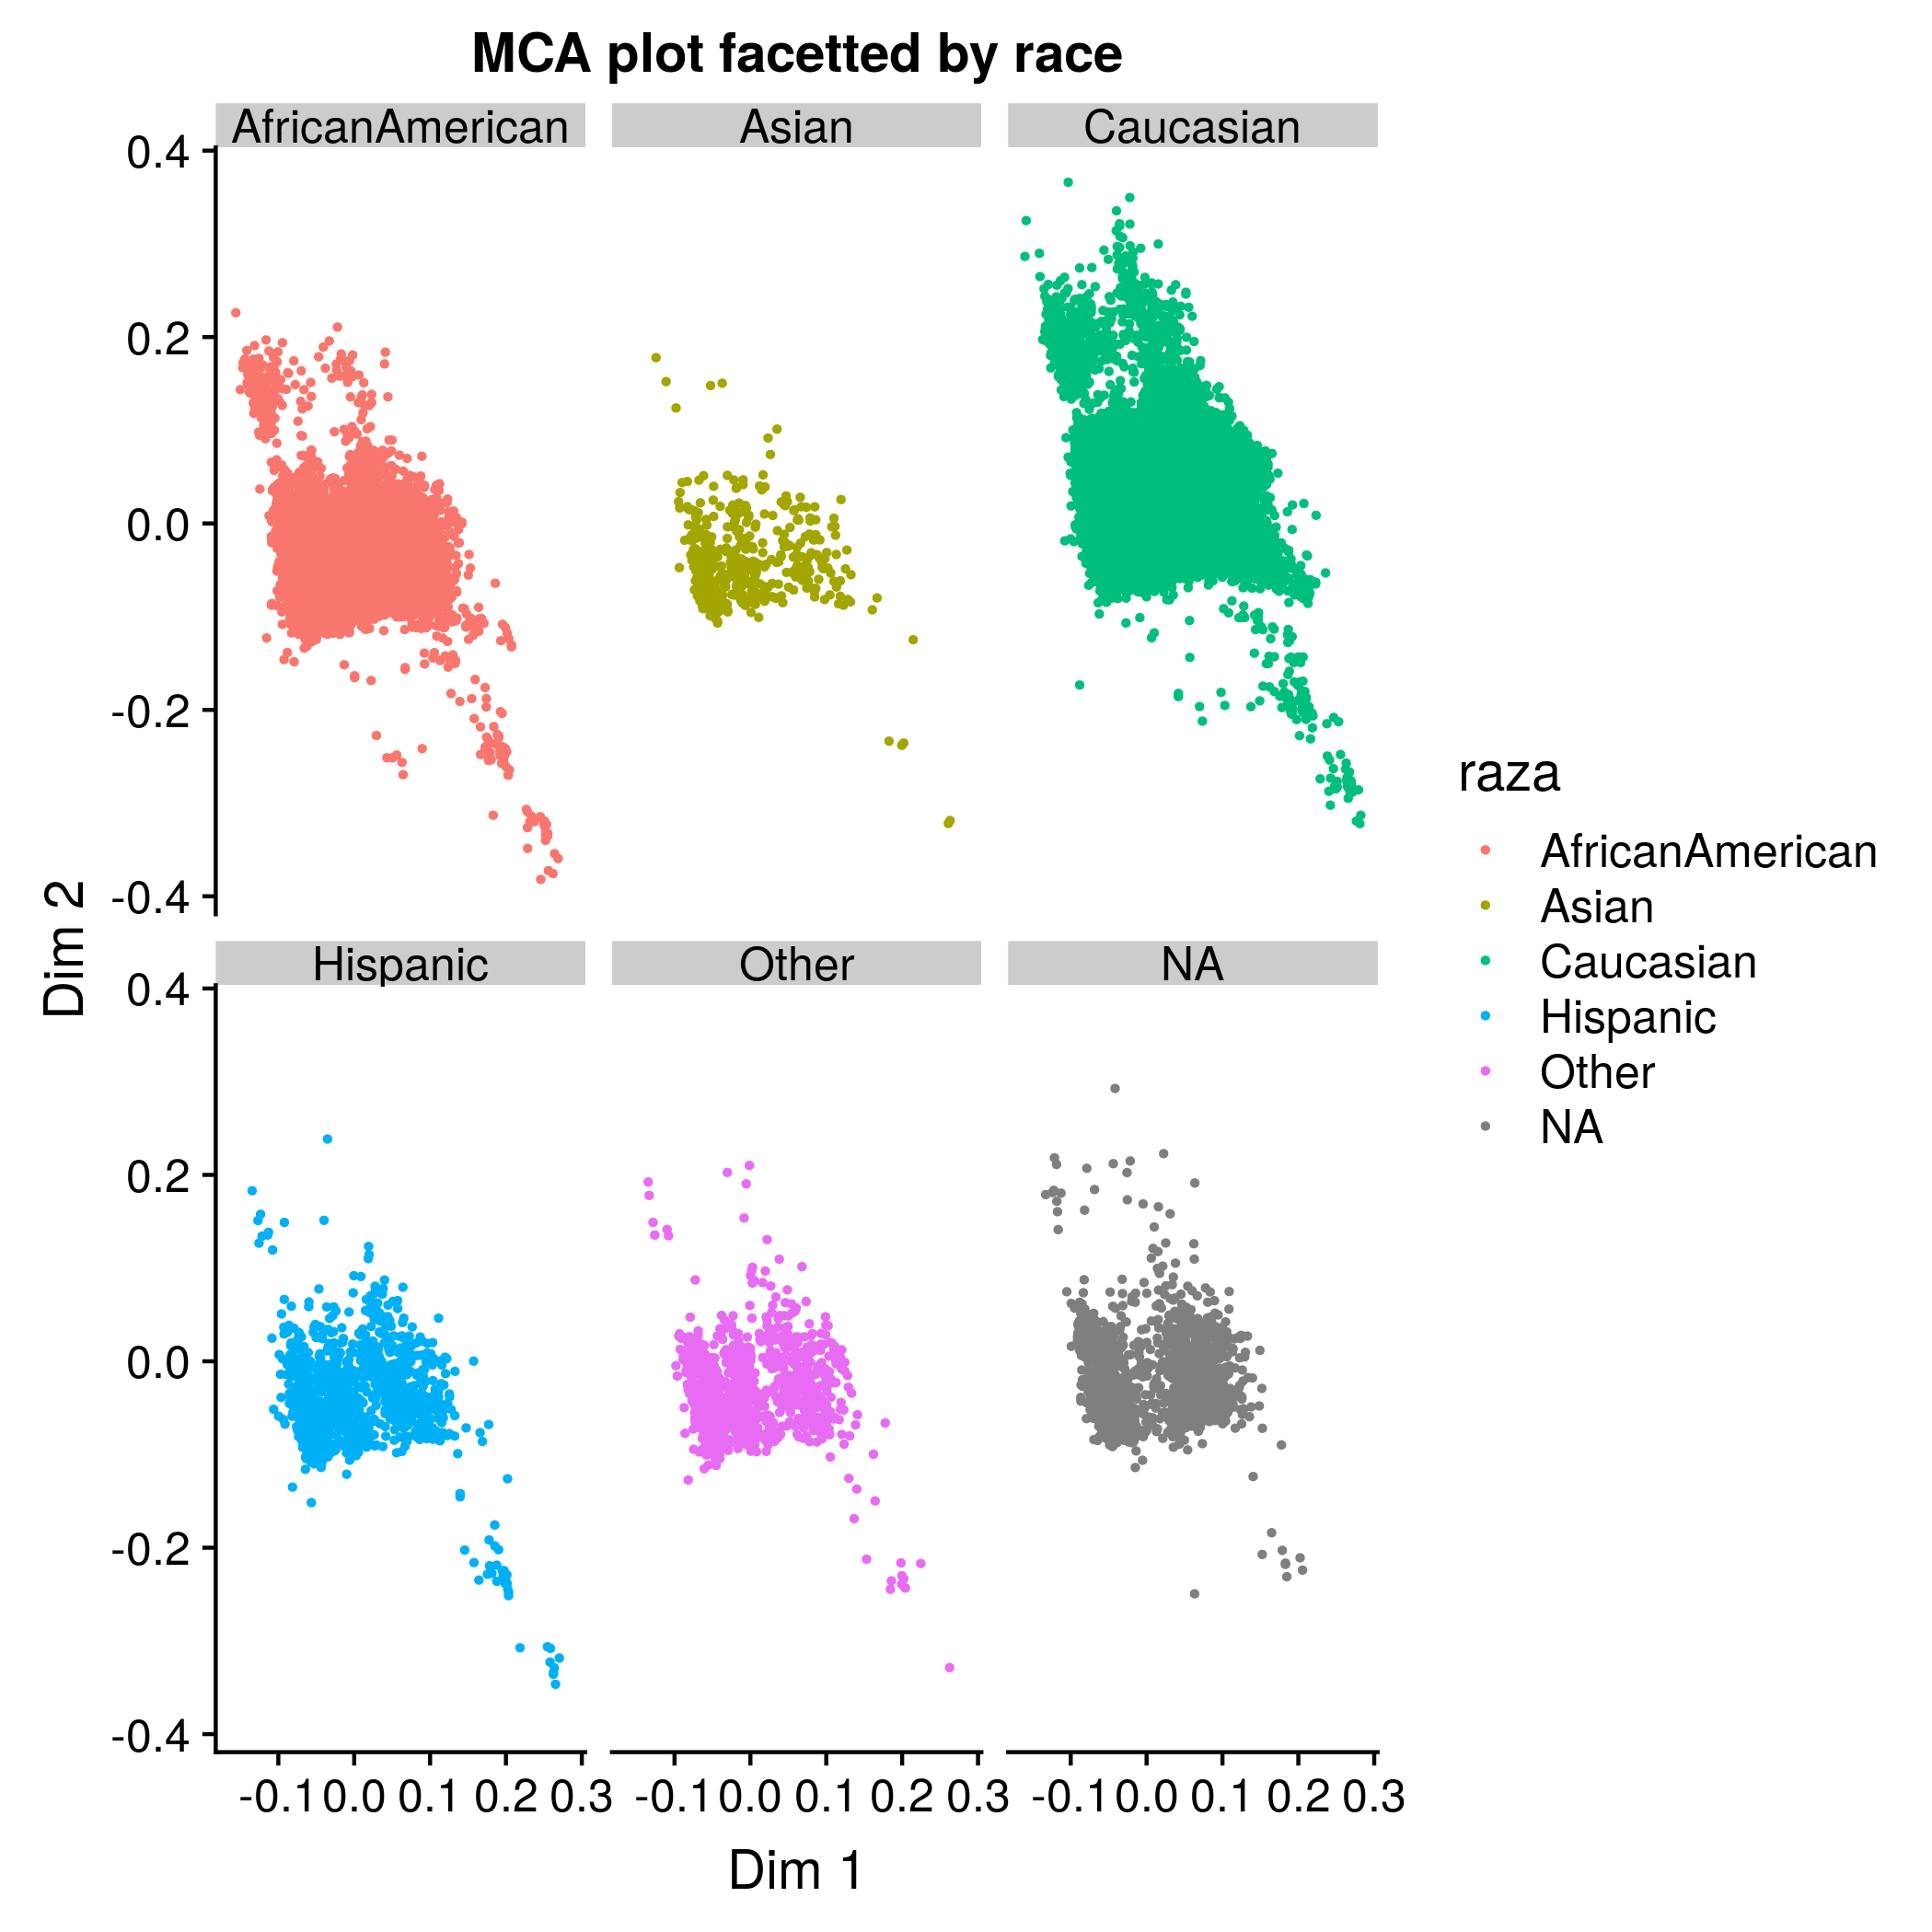
\includegraphics[width=0.5\textwidth]{plots/etiqueta_mca_obs_race_facet}
\end{figure}

\begin{figure}[!h]
\centering
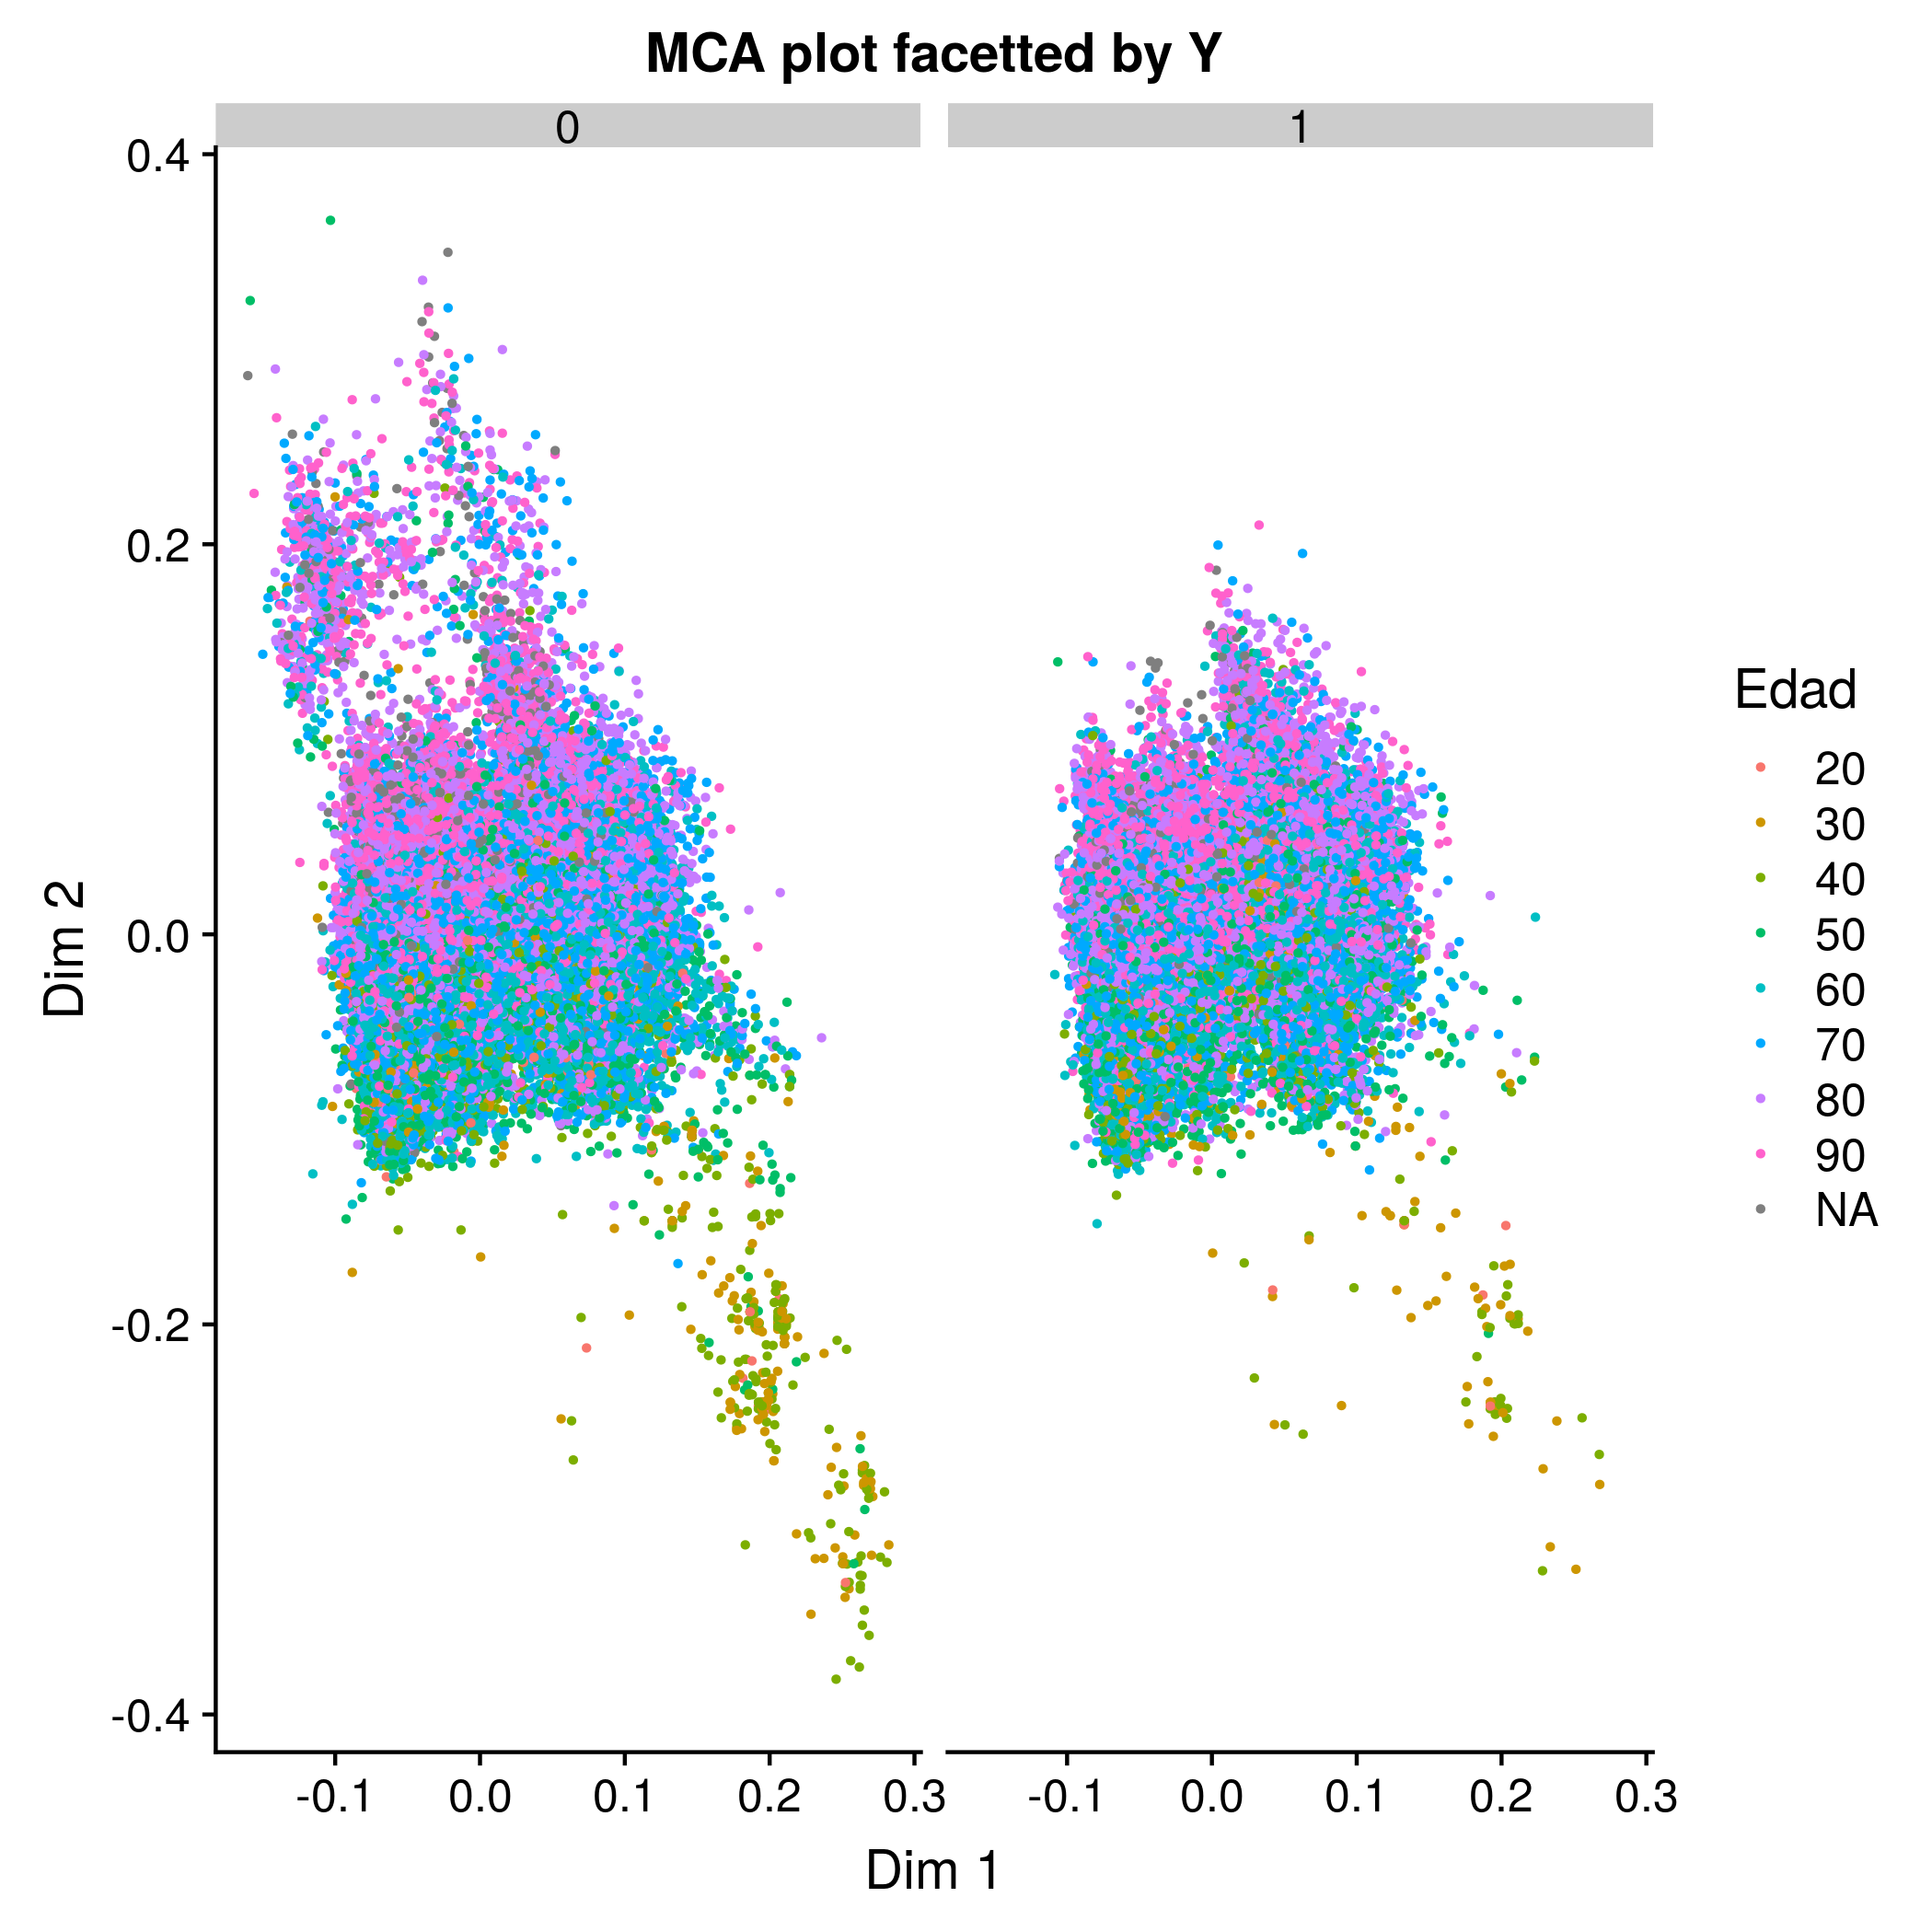
\includegraphics[width=0.5\textwidth]{plots/etiqueta_mca_obs_Y_facet_edad_col}
\end{figure}

\begin{figure}[!h]
\centering
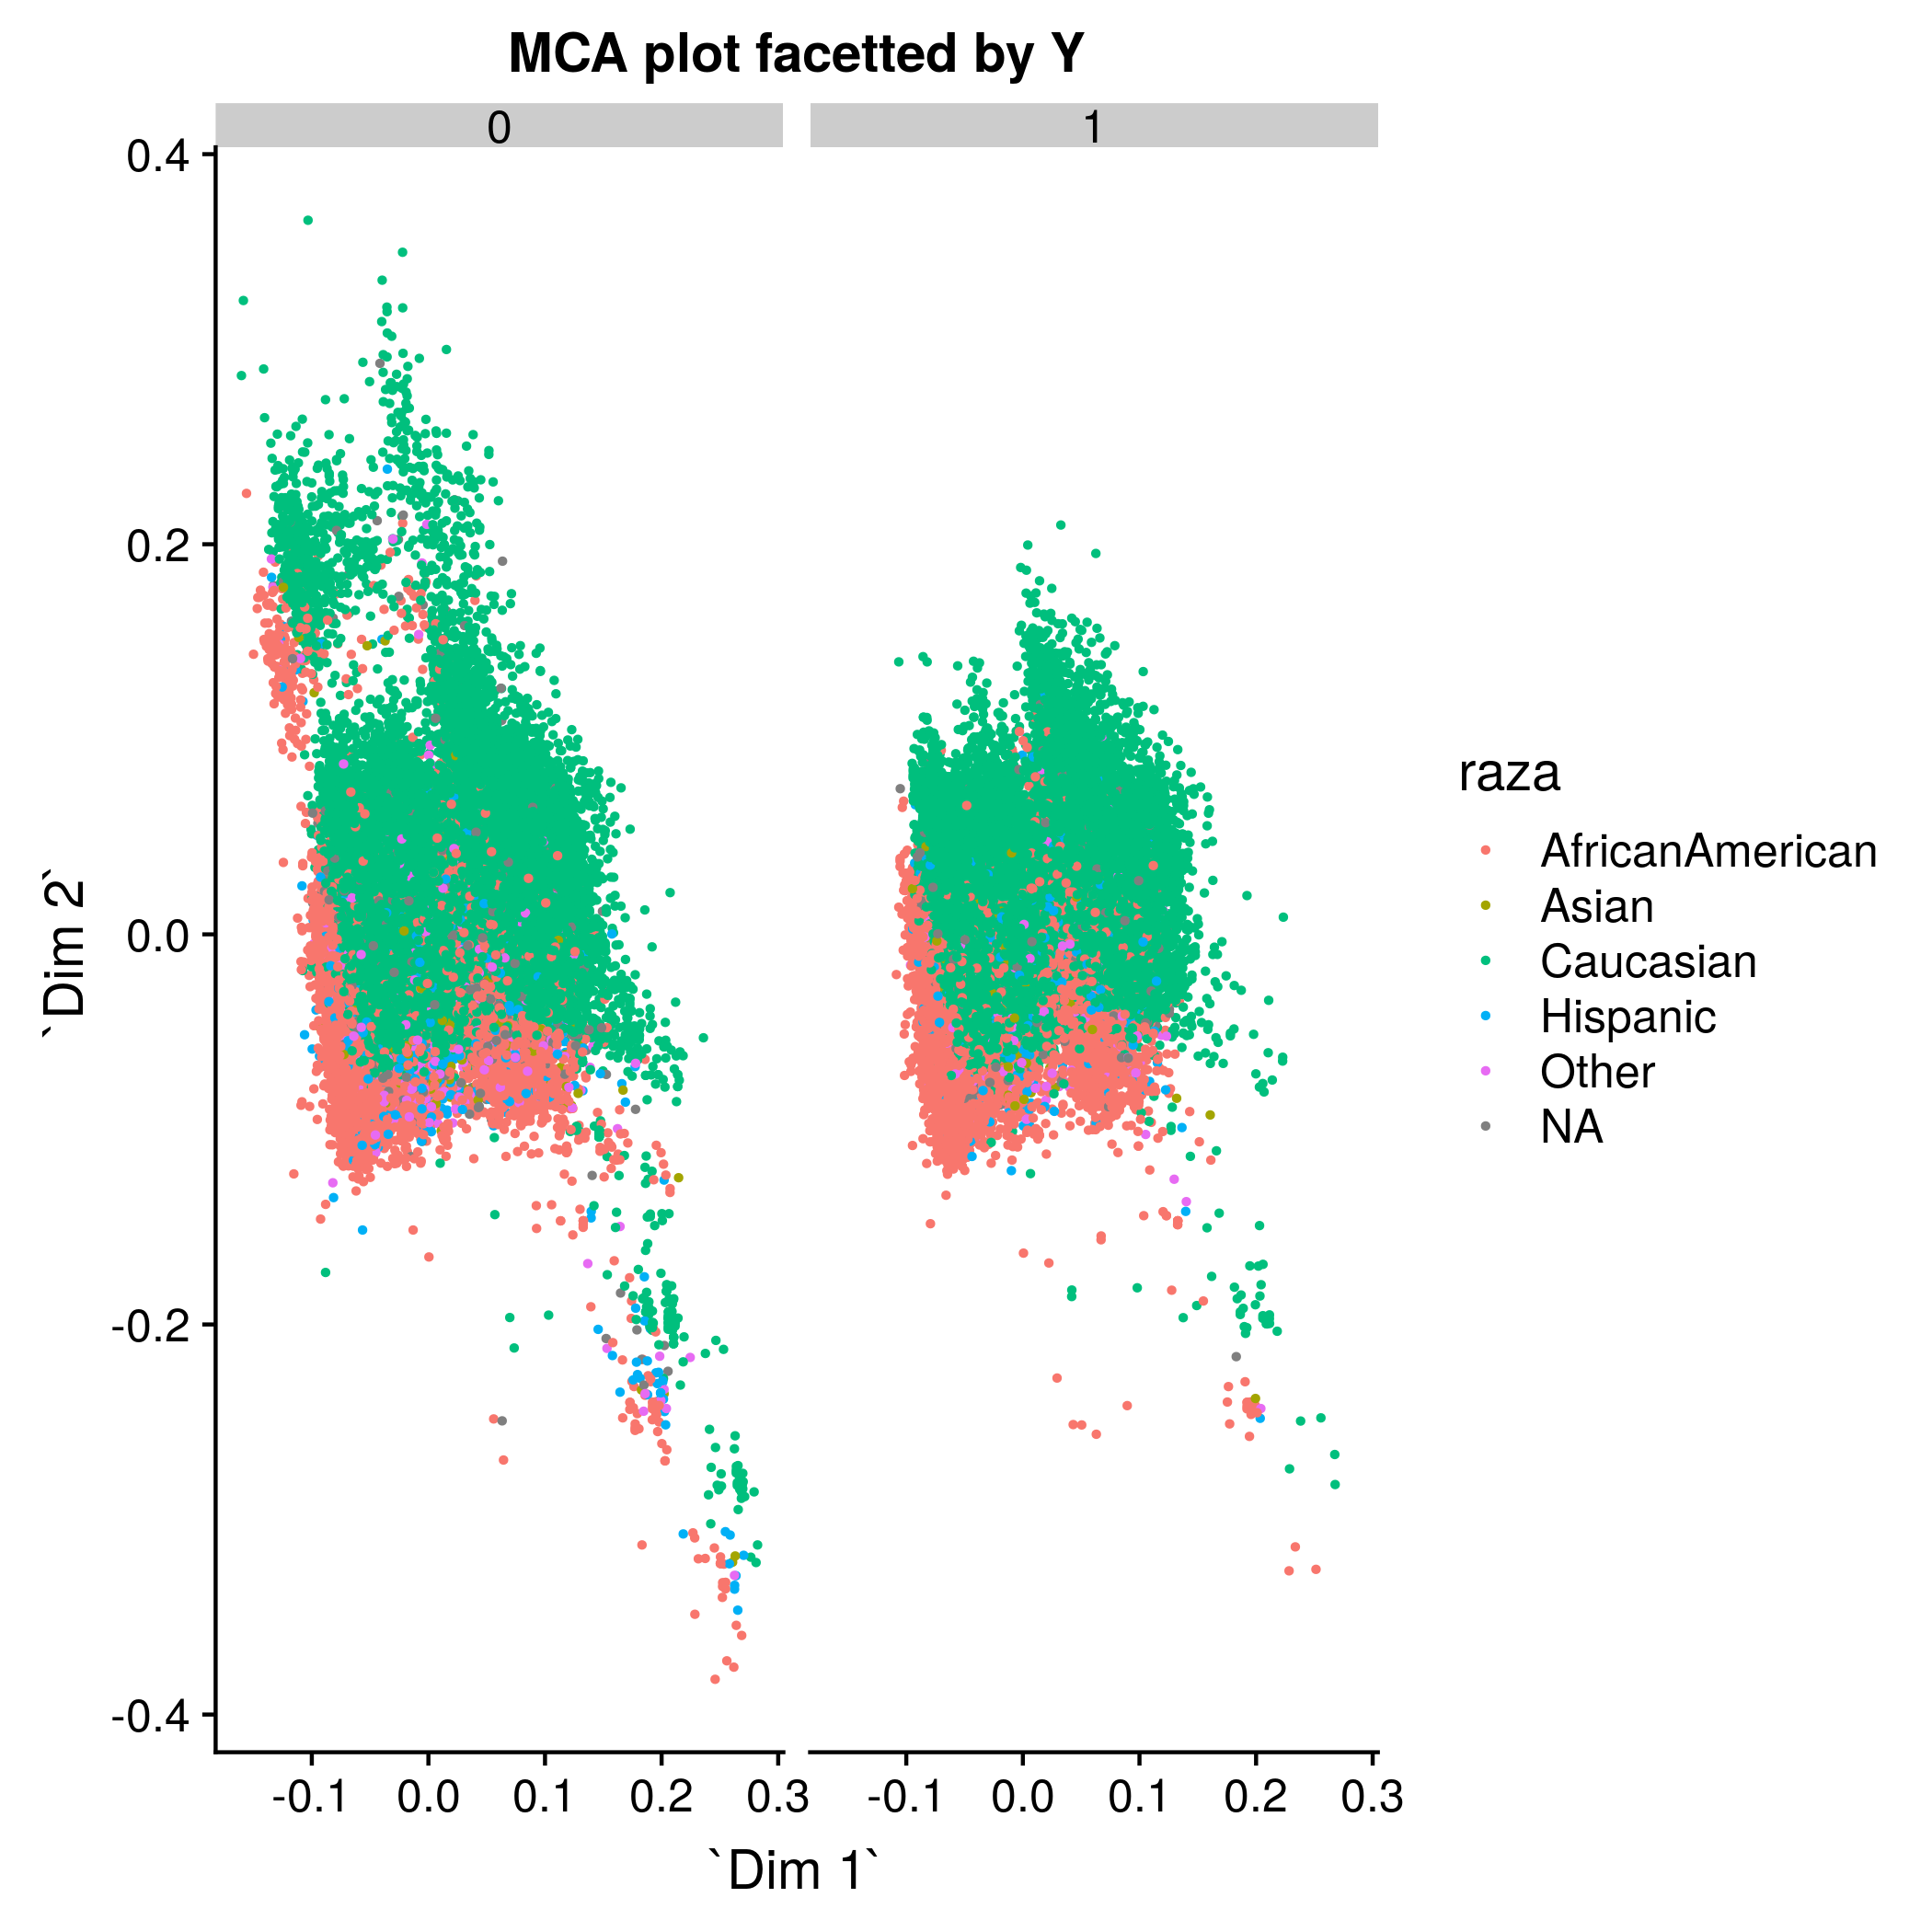
\includegraphics[width=0.5\textwidth]{plots/etiqueta_mca_obs_Y_facet_raza_col}
\end{figure}

\newpage

\section{Appendix B}
\begin{knitrout}
\definecolor{shadecolor}{rgb}{0.969, 0.969, 0.969}\color{fgcolor}\begin{kframe}
\begin{alltt}
\hlstd{preprocess_data} \hlkwb{<-} \hlkwa{function}\hlstd{(}\hlkwc{x_train}\hlstd{,} \hlkwc{x_test}\hlstd{,} \hlkwc{etiquettes} \hlstd{=} \hlnum{FALSE}\hlstd{) \{}

    \hlkwa{if} \hlstd{(etiquettes) \{}
        \hlcom{## Preprocess etiquettes}
        \hlkwd{print}\hlstd{(}\hlstr{"Processing etiquettes"}\hlstd{)}
        \hlstd{train_etiquettes} \hlkwb{<-} \hlstd{x_train[,} \hlkwd{c}\hlstd{(}\hlstr{"etiqueta_1"}\hlstd{,} \hlstr{"etiqueta_2"}\hlstd{,} \hlstr{"etiqueta_3"}\hlstd{)]}
        \hlstd{test_etiquettes} \hlkwb{<-} \hlstd{x_test[,} \hlkwd{c}\hlstd{(}\hlstr{"etiqueta_1"}\hlstd{,} \hlstr{"etiqueta_2"}\hlstd{,} \hlstr{"etiqueta_3"}\hlstd{)]}
        \hlkwd{rownames}\hlstd{(train_etiquettes)} \hlkwb{<-} \hlstd{x_train}\hlopt{$}\hlstd{identificador}
        \hlkwd{rownames}\hlstd{(test_etiquettes)} \hlkwb{<-} \hlstd{x_test}\hlopt{$}\hlstd{identificador}
        \hlstd{unique_etiquettes} \hlkwb{<-} \hlstd{train_etiquettes} \hlopt \hlstd{unlist} \hlopt \hlstd{unique} \hlopt \hlstd{sort}

        \hlstd{etiquettes_template} \hlkwb{<-} \hlkwd{rep}\hlstd{(}\hlnum{0}\hlstd{,} \hlkwd{length}\hlstd{(unique_etiquettes))}
        \hlkwd{names}\hlstd{(etiquettes_template)} \hlkwb{<-} \hlstd{unique_etiquettes}
        \hlstd{etiquettes_proc} \hlkwb{<-} \hlkwd{lapply}\hlstd{(}\hlkwd{list}\hlstd{(}\hlkwc{train} \hlstd{= train_etiquettes,} \hlkwc{test} \hlstd{= test_etiquettes),}
            \hlkwa{function}\hlstd{(}\hlkwc{y}\hlstd{) \{}
                \hlstd{res} \hlkwb{<-} \hlstd{y} \hlopt \hlstd{as.matrix} \hlopt \hlkwd{apply}\hlstd{(.,} \hlnum{1}\hlstd{,} \hlkwa{function}\hlstd{(}\hlkwc{x}\hlstd{) \{}
                  \hlstd{local_count} \hlkwb{<-} \hlkwd{table}\hlstd{(x)}
                  \hlstd{et} \hlkwb{<-} \hlstd{etiquettes_template}
                  \hlcom{# drop any etiquette that's not in the training set}
                  \hlstd{local_count} \hlkwb{<-} \hlstd{local_count[}\hlkwd{names}\hlstd{(local_count)} \hlopt \hlkwd{names}\hlstd{(et)]}
                  \hlstd{et[}\hlkwd{names}\hlstd{(local_count)]} \hlkwb{<-} \hlstd{local_count}
                  \hlkwd{return}\hlstd{(et)}
                \hlstd{\})} \hlopt \hlstd{t} \hlopt \hlstd{unlist}
                \hlkwd{colnames}\hlstd{(res)} \hlkwb{<-} \hlkwd{paste0}\hlstd{(}\hlstr{"et_"}\hlstd{,} \hlkwd{colnames}\hlstd{(res))}
                \hlstd{res} \hlkwb{<-} \hlstd{res} \hlopt \hlkwd{apply}\hlstd{(.,} \hlnum{2}\hlstd{, as.factor)} \hlopt \hlstd{as.data.frame}
                \hlkwd{return}\hlstd{(res)}
            \hlstd{\})}

        \hlcom{# etiquettes_proc$train %>% View OK}
    \hlstd{\}}

    \hlcom{## Preprocess nominals}
    \hlkwd{print}\hlstd{(}\hlstr{"Processing nominals"}\hlstd{)}
    \hlcom{# Drop nominal 4 for now Should remove the last column produced with each nominal}
    \hlstd{train_nominals_one_hot} \hlkwb{<-} \hlstd{x_train} \hlopt \hlkwd{select}\hlstd{(nominal_1}\hlopt{:}\hlstd{nominal_3)} \hlopt \hlkwd{acm.disjonctif}\hlstd{()} \hlopt
        \hlkwd{apply}\hlstd{(.,} \hlnum{2}\hlstd{, as.factor)} \hlopt \hlstd{as.data.frame}
    \hlstd{test_nominals_one_hot} \hlkwb{<-} \hlstd{x_test} \hlopt \hlkwd{select}\hlstd{(nominal_1}\hlopt{:}\hlstd{nominal_3)} \hlopt \hlkwd{acm.disjonctif}\hlstd{()} \hlopt
        \hlkwd{apply}\hlstd{(.,} \hlnum{2}\hlstd{, as.factor)} \hlopt \hlstd{as.data.frame}

    \hlstd{missing_nominal_test} \hlkwb{<-} \hlkwd{colnames}\hlstd{(train_nominals_one_hot)[}\hlopt{!}\hlkwd{colnames}\hlstd{(train_nominals_one_hot)} \hlopt
        \hlkwd{colnames}\hlstd{(test_nominals_one_hot)]}
    \hlstd{missing_test} \hlkwb{<-} \hlkwd{as.data.frame}\hlstd{(}\hlkwd{matrix}\hlstd{(}\hlnum{0}\hlstd{,} \hlkwc{nrow} \hlstd{=} \hlkwd{nrow}\hlstd{(x_test),} \hlkwc{ncol} \hlstd{=} \hlkwd{length}\hlstd{(missing_nominal_test)))}
    \hlkwd{colnames}\hlstd{(missing_test)} \hlkwb{<-} \hlstd{missing_nominal_test}
    \hlstd{test_nominals_one_hot} \hlkwb{<-} \hlkwd{cbind}\hlstd{(test_nominals_one_hot, missing_test)[}\hlkwd{colnames}\hlstd{(train_nominals_one_hot)]}

    \hlstd{nominals_proc} \hlkwb{<-} \hlkwd{list}\hlstd{(}\hlkwc{train} \hlstd{= train_nominals_one_hot,} \hlkwc{test} \hlstd{= test_nominals_one_hot)}

    \hlstd{nominals_proc}\hlopt{$}\hlstd{train} \hlopt \hlstd{class}
    \hlcom{# OK}

    \hlcom{## Preprocess drugs (farmacos)}
    \hlkwd{print}\hlstd{(}\hlstr{"Processing drugs"}\hlstd{)}

    \hlstd{train_drugs} \hlkwb{<-} \hlstd{x_train[,} \hlkwd{grep}\hlstd{(}\hlkwc{pattern} \hlstd{=} \hlstr{"farmaco"}\hlstd{,} \hlkwc{x} \hlstd{=} \hlkwd{colnames}\hlstd{(x_train))]}
    \hlstd{test_drugs} \hlkwb{<-} \hlstd{x_test[,} \hlkwd{grep}\hlstd{(}\hlkwc{pattern} \hlstd{=} \hlstr{"farmaco"}\hlstd{,} \hlkwc{x} \hlstd{=} \hlkwd{colnames}\hlstd{(x_test))]}

    \hlcom{# Drop drugs with no variability (non-informative)}
    \hlstd{train_drugs} \hlkwb{<-} \hlstd{train_drugs[, train_drugs} \hlopt \hlkwd{apply}\hlstd{(.,} \hlnum{2}\hlstd{,} \hlkwa{function}\hlstd{(}\hlkwc{x}\hlstd{)} \hlkwd{length}\hlstd{(}\hlkwd{unique}\hlstd{(x)))} \hlopt{>}
        \hlnum{1}\hlstd{]}
    \hlstd{test_drugs} \hlkwb{<-} \hlstd{test_drugs[,} \hlkwd{colnames}\hlstd{(train_drugs)]}

    \hlcom{# Replace strings with integer}
    \hlstd{drugs_proc} \hlkwb{<-} \hlkwd{list}\hlstd{(}\hlkwc{train} \hlstd{= train_drugs,} \hlkwc{test} \hlstd{= test_drugs)} \hlopt \hlkwd{lapply}\hlstd{(}\hlkwa{function}\hlstd{(}\hlkwc{x}\hlstd{) \{}
        \hlstd{x[x} \hlopt{==} \hlstr{"No"}\hlstd{]} \hlkwb{<-} \hlstr{"-1"}
        \hlstd{x[x} \hlopt{==} \hlstr{"Down"}\hlstd{]} \hlkwb{<-} \hlstr{"0"}
        \hlstd{x[x} \hlopt{==} \hlstr{"Steady"}\hlstd{]} \hlkwb{<-} \hlstr{"1"}
        \hlstd{x[x} \hlopt{==} \hlstr{"Up"}\hlstd{]} \hlkwb{<-} \hlstr{"2"}
        \hlstd{x} \hlkwb{<-} \hlstd{x} \hlopt \hlkwd{apply}\hlstd{(.,} \hlnum{2}\hlstd{, as.integer)} \hlopt \hlstd{as.data.frame}
    \hlstd{\})}

    \hlstd{drugs_proc}\hlopt{$}\hlstd{train} \hlopt \hlstd{class}

    \hlcom{## Preprocess ordinal}
    \hlkwd{print}\hlstd{(}\hlstr{"Processing ordinals"}\hlstd{)}

    \hlstd{train_ordinal} \hlkwb{<-} \hlstd{x_train} \hlopt \hlkwd{select}\hlstd{(ordinal_1}\hlopt{:}\hlstd{ordinal_2)}
    \hlstd{test_ordinal} \hlkwb{<-} \hlstd{x_test} \hlopt \hlkwd{select}\hlstd{(ordinal_1}\hlopt{:}\hlstd{ordinal_2)}
    \hlstd{ordinals_proc} \hlkwb{<-} \hlkwd{lapply}\hlstd{(}\hlkwd{list}\hlstd{(}\hlkwc{train} \hlstd{= train_ordinal,} \hlkwc{test} \hlstd{= test_ordinal),} \hlkwa{function}\hlstd{(}\hlkwc{x}\hlstd{) \{}
        \hlstd{x[x} \hlopt{==} \hlstr{"None"}\hlstd{]} \hlkwb{<-} \hlstr{"0"}
        \hlstd{x[x} \hlopt{==} \hlstr{"Norm"}\hlstd{]} \hlkwb{<-} \hlstr{"1"}
        \hlstd{x[x} \hlopt{==} \hlstr{">7"} \hlopt{|} \hlstd{x} \hlopt{==} \hlstr{">200"}\hlstd{]} \hlkwb{<-} \hlstr{"2"}
        \hlstd{x[x} \hlopt{==} \hlstr{">8"} \hlopt{|} \hlstd{x} \hlopt{==} \hlstr{">300"}\hlstd{]} \hlkwb{<-} \hlstr{"3"}
        \hlstd{x} \hlkwb{<-} \hlstd{x} \hlopt \hlkwd{apply}\hlstd{(.,} \hlnum{2}\hlstd{, as.integer)} \hlopt \hlstd{as.data.frame}
        \hlstd{x}
    \hlstd{\})}

    \hlstd{ordinals_proc}\hlopt{$}\hlstd{train} \hlopt \hlstd{class}


    \hlcom{## Preprocess binary}
    \hlkwd{print}\hlstd{(}\hlstr{"Processing binaries"}\hlstd{)}

    \hlstd{train_binary} \hlkwb{<-} \hlstd{x_train} \hlopt \hlkwd{select}\hlstd{(binary_1}\hlopt{:}\hlstd{binary_3)} \hlopt \hlkwd{apply}\hlstd{(.,} \hlnum{2}\hlstd{,} \hlkwa{function}\hlstd{(}\hlkwc{x}\hlstd{)} \hlkwd{as.factor}\hlstd{(}\hlkwd{as.integer}\hlstd{(}\hlkwd{as.factor}\hlstd{(x))} \hlopt{-}
        \hlnum{1}\hlstd{))} \hlopt \hlstd{as.data.frame}
    \hlstd{test_binary} \hlkwb{<-} \hlstd{x_test} \hlopt \hlkwd{select}\hlstd{(binary_1}\hlopt{:}\hlstd{binary_3)} \hlopt \hlkwd{apply}\hlstd{(.,} \hlnum{2}\hlstd{,} \hlkwa{function}\hlstd{(}\hlkwc{x}\hlstd{)} \hlkwd{as.factor}\hlstd{(}\hlkwd{as.integer}\hlstd{(}\hlkwd{as.factor}\hlstd{(x))} \hlopt{-}
        \hlnum{1}\hlstd{))} \hlopt \hlstd{as.data.frame}
    \hlstd{binary_proc} \hlkwb{<-} \hlkwd{list}\hlstd{(}\hlkwc{train} \hlstd{= train_binary,} \hlkwc{test} \hlstd{= test_binary)}

    \hlstd{binary_proc}\hlopt{$}\hlstd{train} \hlopt \hlstd{class}

    \hlcom{## Preprocess counter}
    \hlkwd{print}\hlstd{(}\hlstr{"Processing counters"}\hlstd{)}

    \hlstd{counter_proc} \hlkwb{<-} \hlkwd{list}\hlstd{(}\hlkwc{train} \hlstd{= x_train} \hlopt \hlkwd{select}\hlstd{(counter_1}\hlopt{:}\hlstd{counter_7),} \hlkwc{test} \hlstd{= x_test} \hlopt
        \hlkwd{select}\hlstd{(counter_1}\hlopt{:}\hlstd{counter_7))}
    \hlstd{counter_proc}\hlopt{$}\hlstd{train} \hlopt \hlstd{class}

    \hlcom{## Preprocess race}
    \hlkwd{print}\hlstd{(}\hlstr{"Processing race"}\hlstd{)}

    \hlstd{race_proc} \hlkwb{<-} \hlkwd{list}\hlstd{(}\hlkwc{train} \hlstd{= x_train} \hlopt \hlkwd{select}\hlstd{(raza)} \hlopt \hlkwd{acm.disjonctif}\hlstd{()} \hlopt \hlkwd{apply}\hlstd{(.,}
        \hlnum{2}\hlstd{, as.factor)} \hlopt \hlstd{as.data.frame,} \hlkwc{test} \hlstd{= x_test} \hlopt \hlkwd{select}\hlstd{(raza)} \hlopt \hlkwd{acm.disjonctif}\hlstd{()} \hlopt
        \hlkwd{apply}\hlstd{(.,} \hlnum{2}\hlstd{, as.factor)} \hlopt \hlstd{as.data.frame)}

    \hlstd{race_proc}\hlopt{$}\hlstd{train} \hlopt \hlstd{class}

    \hlcom{## Preprocess sex}
    \hlkwd{print}\hlstd{(}\hlstr{"Processing sex"}\hlstd{)}

    \hlstd{sex_proc} \hlkwb{<-} \hlkwd{list}\hlstd{(}\hlkwc{train} \hlstd{= x_train} \hlopt \hlkwd{select}\hlstd{(sexo)} \hlopt \hlkwd{apply}\hlstd{(.,} \hlnum{2}\hlstd{,} \hlkwa{function}\hlstd{(}\hlkwc{x}\hlstd{)} \hlkwd{as.factor}\hlstd{(}\hlkwd{as.integer}\hlstd{(}\hlkwd{as.factor}\hlstd{(x))} \hlopt{-}
        \hlnum{1}\hlstd{))} \hlopt \hlstd{as.data.frame,} \hlkwc{test} \hlstd{= x_test} \hlopt \hlkwd{select}\hlstd{(sexo)} \hlopt \hlkwd{apply}\hlstd{(.,} \hlnum{2}\hlstd{,} \hlkwa{function}\hlstd{(}\hlkwc{x}\hlstd{)} \hlkwd{as.factor}\hlstd{(}\hlkwd{as.integer}\hlstd{(}\hlkwd{as.factor}\hlstd{(x))} \hlopt{-}
        \hlnum{1}\hlstd{))} \hlopt \hlstd{as.data.frame)}

    \hlcom{## Preprocess age}
    \hlkwd{print}\hlstd{(}\hlstr{"Processing age"}\hlstd{)}

    \hlstd{train_age} \hlkwb{<-} \hlstd{x_train}\hlopt{$}\hlstd{edad_integer}
    \hlstd{train_age_mean} \hlkwb{<-} \hlkwd{mean}\hlstd{(train_age,} \hlkwc{na.rm} \hlstd{= T)}
    \hlstd{train_age[}\hlkwd{is.na}\hlstd{(train_age)]} \hlkwb{<-} \hlstd{train_age_mean}
    \hlstd{test_age} \hlkwb{<-} \hlstd{x_test}\hlopt{$}\hlstd{edad_integer}
    \hlstd{test_age[}\hlkwd{is.na}\hlstd{(test_age)]} \hlkwb{<-} \hlstd{train_age_mean}

    \hlstd{age_proc} \hlkwb{<-} \hlkwd{list}\hlstd{(}\hlkwc{train} \hlstd{=} \hlkwd{data.frame}\hlstd{(}\hlkwc{edad_integer} \hlstd{= train_age),} \hlkwc{test} \hlstd{=} \hlkwd{data.frame}\hlstd{(}\hlkwc{edad_integer} \hlstd{= test_age))}

    \hlstd{datasets} \hlkwb{<-} \hlkwd{c}\hlstd{(}\hlstr{"train"}\hlstd{,} \hlstr{"test"}\hlstd{)}
    \hlkwa{if} \hlstd{(etiquettes) \{}
        \hlstd{processed_datasets} \hlkwb{<-} \hlkwd{lapply}\hlstd{(datasets,} \hlkwa{function}\hlstd{(}\hlkwc{x}\hlstd{) \{}
            \hlkwd{cbind}\hlstd{(race_proc[[x]], sex_proc[[x]], age_proc[[x]], nominals_proc[[x]],}
                \hlstd{counter_proc[[x]], drugs_proc[[x]], ordinals_proc[[x]], binary_proc[[x]],}
                \hlstd{etiquettes_proc[[x]])}
        \hlstd{\})}
    \hlstd{\}} \hlkwa{else} \hlstd{\{}
        \hlstd{processed_datasets} \hlkwb{<-} \hlkwd{lapply}\hlstd{(datasets,} \hlkwa{function}\hlstd{(}\hlkwc{x}\hlstd{) \{}
            \hlkwd{cbind}\hlstd{(race_proc[[x]], sex_proc[[x]], age_proc[[x]], nominals_proc[[x]],}
                \hlstd{counter_proc[[x]], drugs_proc[[x]], ordinals_proc[[x]], binary_proc[[x]])}
        \hlstd{\})}
    \hlstd{\}}

    \hlkwd{names}\hlstd{(processed_datasets)} \hlkwb{<-} \hlstd{datasets}
    \hlkwd{return}\hlstd{(processed_datasets)}
\hlstd{\}}
\end{alltt}
\end{kframe}
\end{knitrout}

\end{document}
